\documentclass{scrartcl}
\usepackage{graphicx} 
\usepackage[utf8]{inputenc}
\usepackage[T1]{fontenc}
\usepackage[ngerman]{babel}
\usepackage{amsmath}
\usepackage{amssymb}
\usepackage{graphicx}
\usepackage[dvipsnames]{xcolor} 
\usepackage{array,mathtools}
\usepackage{color}
\usepackage{hhline}
\usepackage{tikz}
\usetikzlibrary{arrows,shapes,snakes,automata,backgrounds,petri}
\usepackage{enumitem}
\usepackage{float}
\usepackage{smartdiagram}
\usepackage[automark]{scrpage2}
\usepackage{pgfplots}
\pgfplotsset{compat=1.8}
\usepgfplotslibrary{statistics}
 
\newcommand{\BMM}{\texttt{\textit{Bodensee Mau Mau}}}
 
\title{Abschlussdokumentation}
\author{Ulli Hagenlocher, Marc Krause, Christoph Schröder}
\date{\today}


\begin{document} 
\maketitle
\section*{Aufgabe 1: Projektbeschreibung}
\subsection*{a) Überblick}
Unsere Idee ist das selbsterdachte Spiel \BMM vorzustellen und zu erklären. Die Website richtet sich an Personen aller Altersgruppen ab 12 Jahren, da die Regeln relativ komplex sind. Speziell an jugendliche Personen (da es z. B. auch eine Trinkspielvariante gibt) die ein neues, komplexes Kartenspiel suchen, ohne Geld dafür ausgeben zu wollen. Doch auch Personen, die das Spiel bereits kennen und bestimmte Regeln nachschlagen möchten. Unsere \textbf{Zielsetzung} ist die Verbreitung dieses (für uns) tollen Kartenspiels.
\subsection*{b) Szenarien} 
\begin{description}
\item[Szenario 1:]
Der Nutzer sucht bei einer großen Suchmaschine nach einem Partyspiel. Der erste Treffer führt auf unsere Seite. Der Nutzer gewinnt durch die Übersicht an Interesse, so dass er mit seinen Freunden das Spiel ausprobiert.
\item[Szenario 2:]
Der Nutzer kennt das Spiel bereits, hat aber noch Fragen und besucht daher die Website. Dort kann er im Regelwerk offene Fragen klären.

\item[Szenario 3:]
Der Nutzer kennt das Spiel bereits. Er möchte durch regelmäßiges Aufsuchen der Website auf dem aktuellem Stand bleiben.
\end{description}

 \section*{Aufgabe 2: Entwicklung einer Navigationsstruktur} 
 \subsection*{1. Funktionalitäten/Inhalte:} 
 Alle Regeln + Varianten, einen Downloadbereich (für z.B das Regelwerk), einen Bereich mit aktuellen Änderungen/Ergänzungen, ein Impressum, die Geschichte hinter dem Spiel (wie ist es entstanden?), eine Übersicht für Erstbesucher (auf der Startseite)
\subsection*{2. Oberbegriffe:}  
 \begin{itemize}
 \item Startseite
 \item News
 \item Regeln
 \begin{itemize}
 \item Varianten
 \end{itemize}
 \item Geschichte
 \item Impressum
 \item Downloads
 \end{itemize}
 \subsection*{3. Schema}
 \begin{figure}[H]
 \centering
 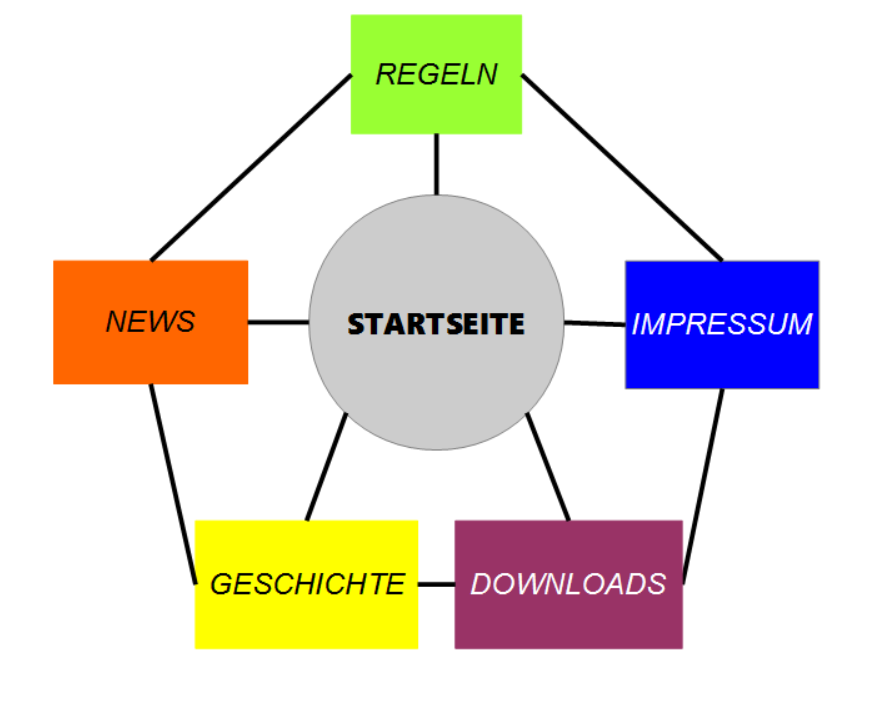
\includegraphics[width=0.7\textwidth]{schema.png}
\caption{Graphische Darstellung der Navigation}
\end{figure} 
Über eine Navigationsleiste, die auf jeder Seite enthalten ist, kann man zu: \textit{Startseite}, \textit{Regeln}, \textit{News}, \textit{Geschichte} und \textit{Downloads}. Im Footer kann der Nutzer das  \textit{Impressum} erreichen.\\
 Ausgangspunkt ist die Startseite mit einer kurzen Information, also einer Übersicht, zum Spiel. Über die Übersicht gelangt der Nutzer durch einen Button direkt zu den \textit{Regeln} und kann über die Navigationsleiste weiter zu \textit{News}, \textit{Geschichte} und \textit{Downloads}. 
 Geht er zu \textit{Regeln}, hat er noch zusätzlich die Möglichkeit zu den einzelnen Unterpunkten zu springen (durch möglicherweise eine zusätzliche Navigation). Auf der Seite \textit{News} hat er auch die Möglichkeit direkt zu bestimmten Punkten von \textit{Regeln}, z. B. einer neuen Regeln, zu gelangen.

\section*{Aufgabe 3: Strukturierung der Nutzeroberfläche}

 \subsection*{1. Entwurf}
  \begin{figure}[H]
 \centering
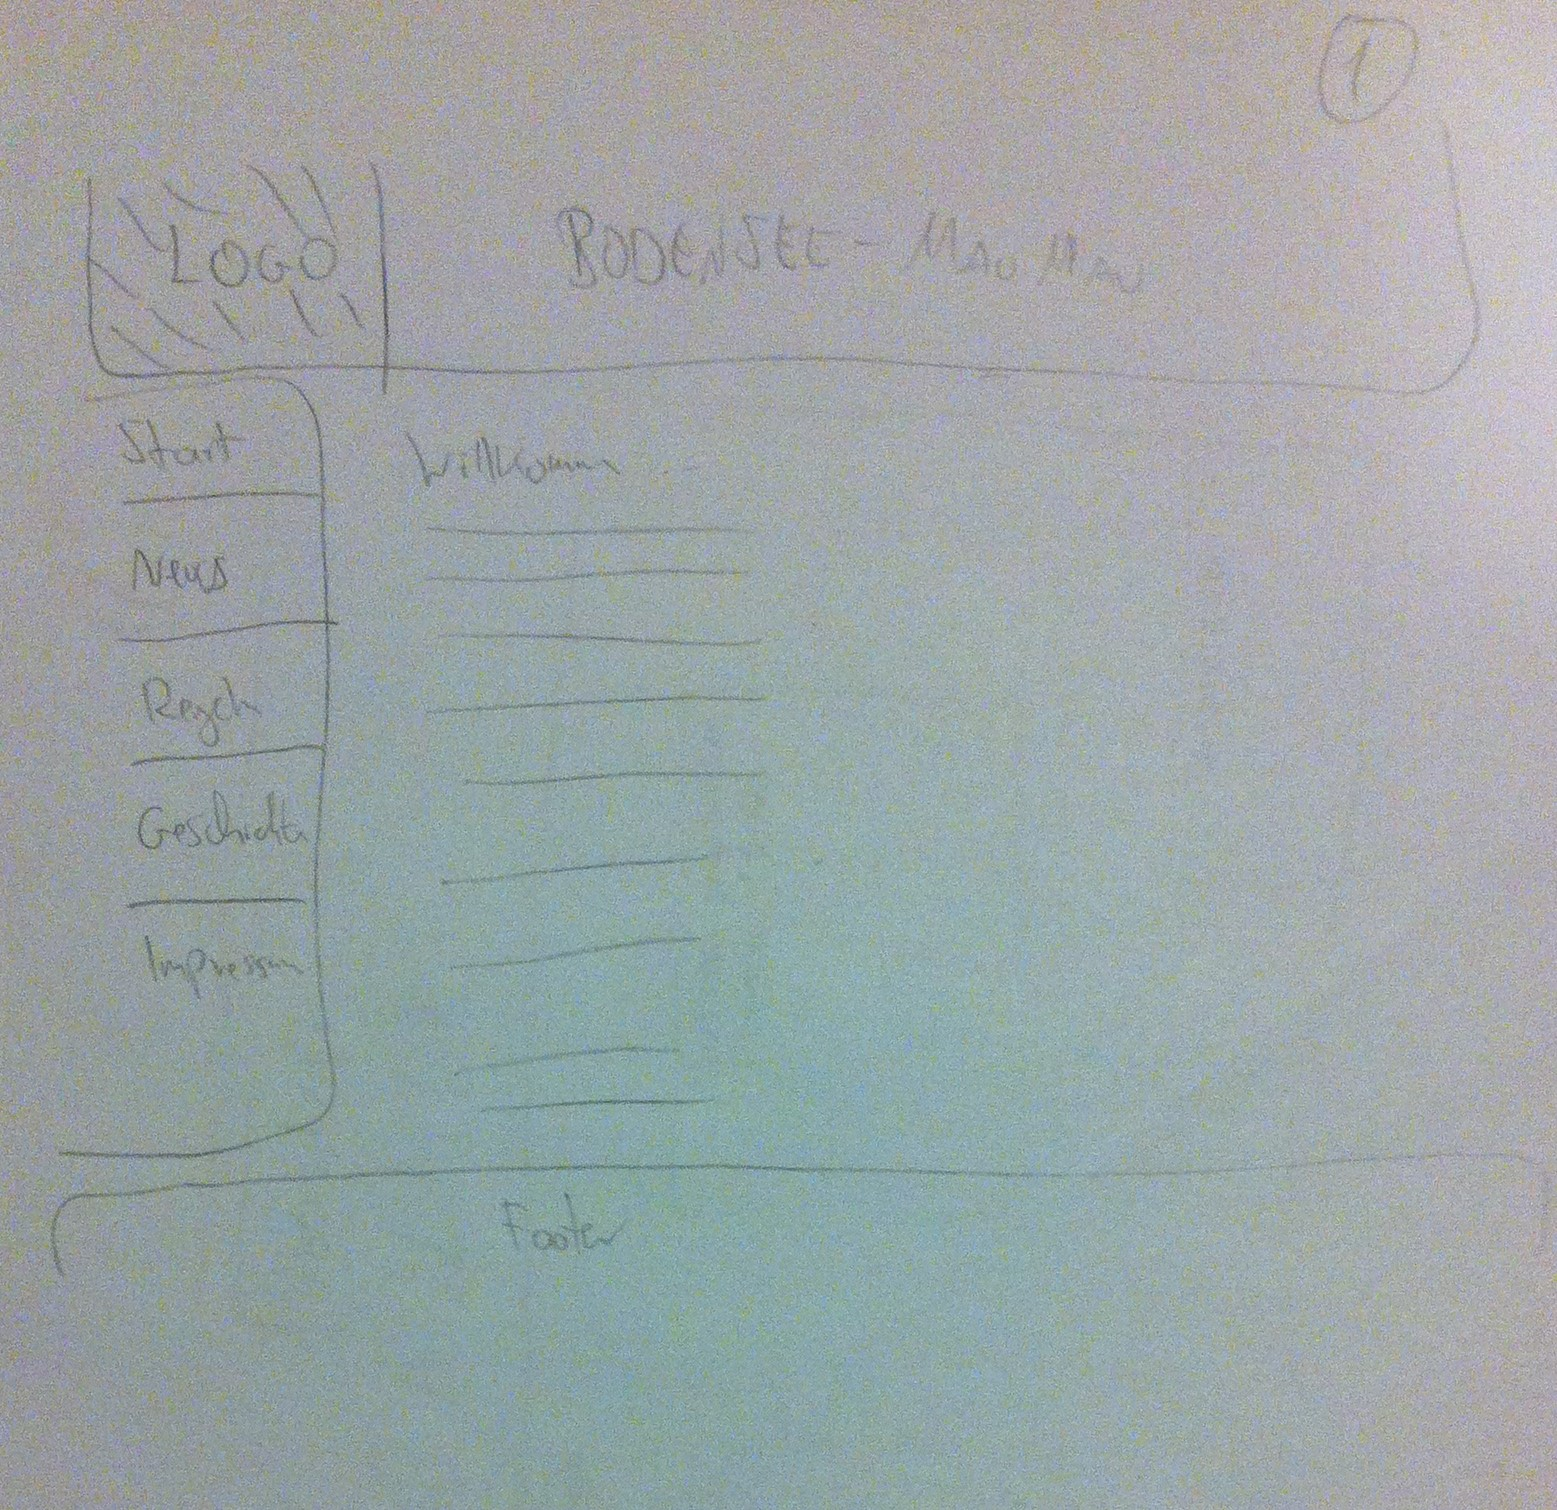
\includegraphics[width=0.7\textwidth]{Version1.jpg}
\caption{Entwurf 1, Christoph}
\end{figure}
 \begin{description}
 \item[Vorteile:]
 Einfache Struktur, übersichtlich, benutzerfreundlich
 \item[Nachteile:] Nicht besonders anprechend, veraltetes Design bezüglich der Navigationsleiste
\end{description}
 
 \subsection*{2. Entwurf}
  \begin{figure}[H]
 \centering
 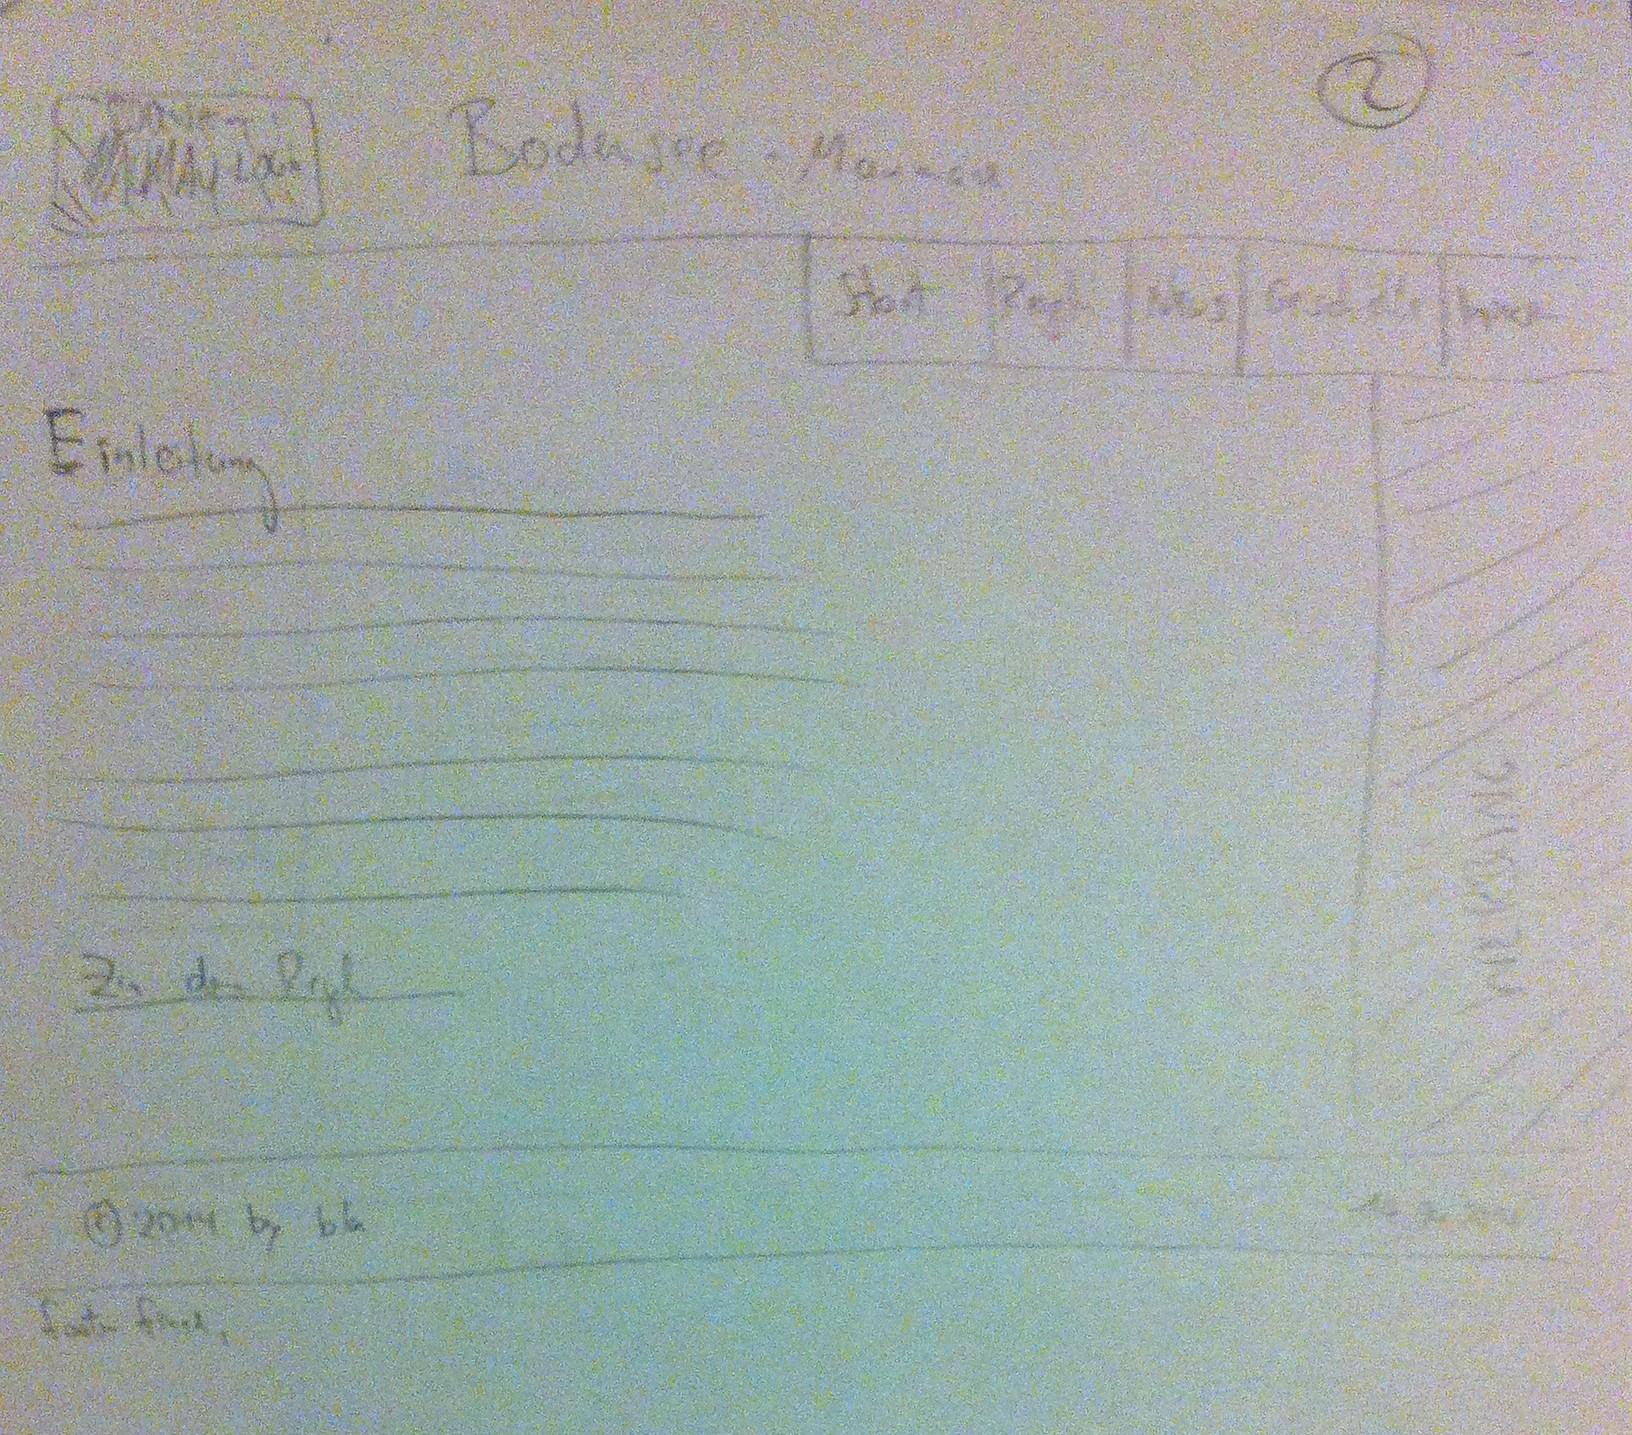
\includegraphics[width=0.7\textwidth]{Version2.jpg}
\caption{Entwurf 2, Christoph}
\end{figure} 
 \begin{description}
 \item[Vorteile:] Aufmerkskeitserregendes Design
 \item[Nachteile:] Bedingt benutzerfreundlich, Navigationsleiste könnte zu Verwirrung führen
 \end{description}

 \subsection*{3. Entwurf}
  \begin{figure}[H]
 \centering
  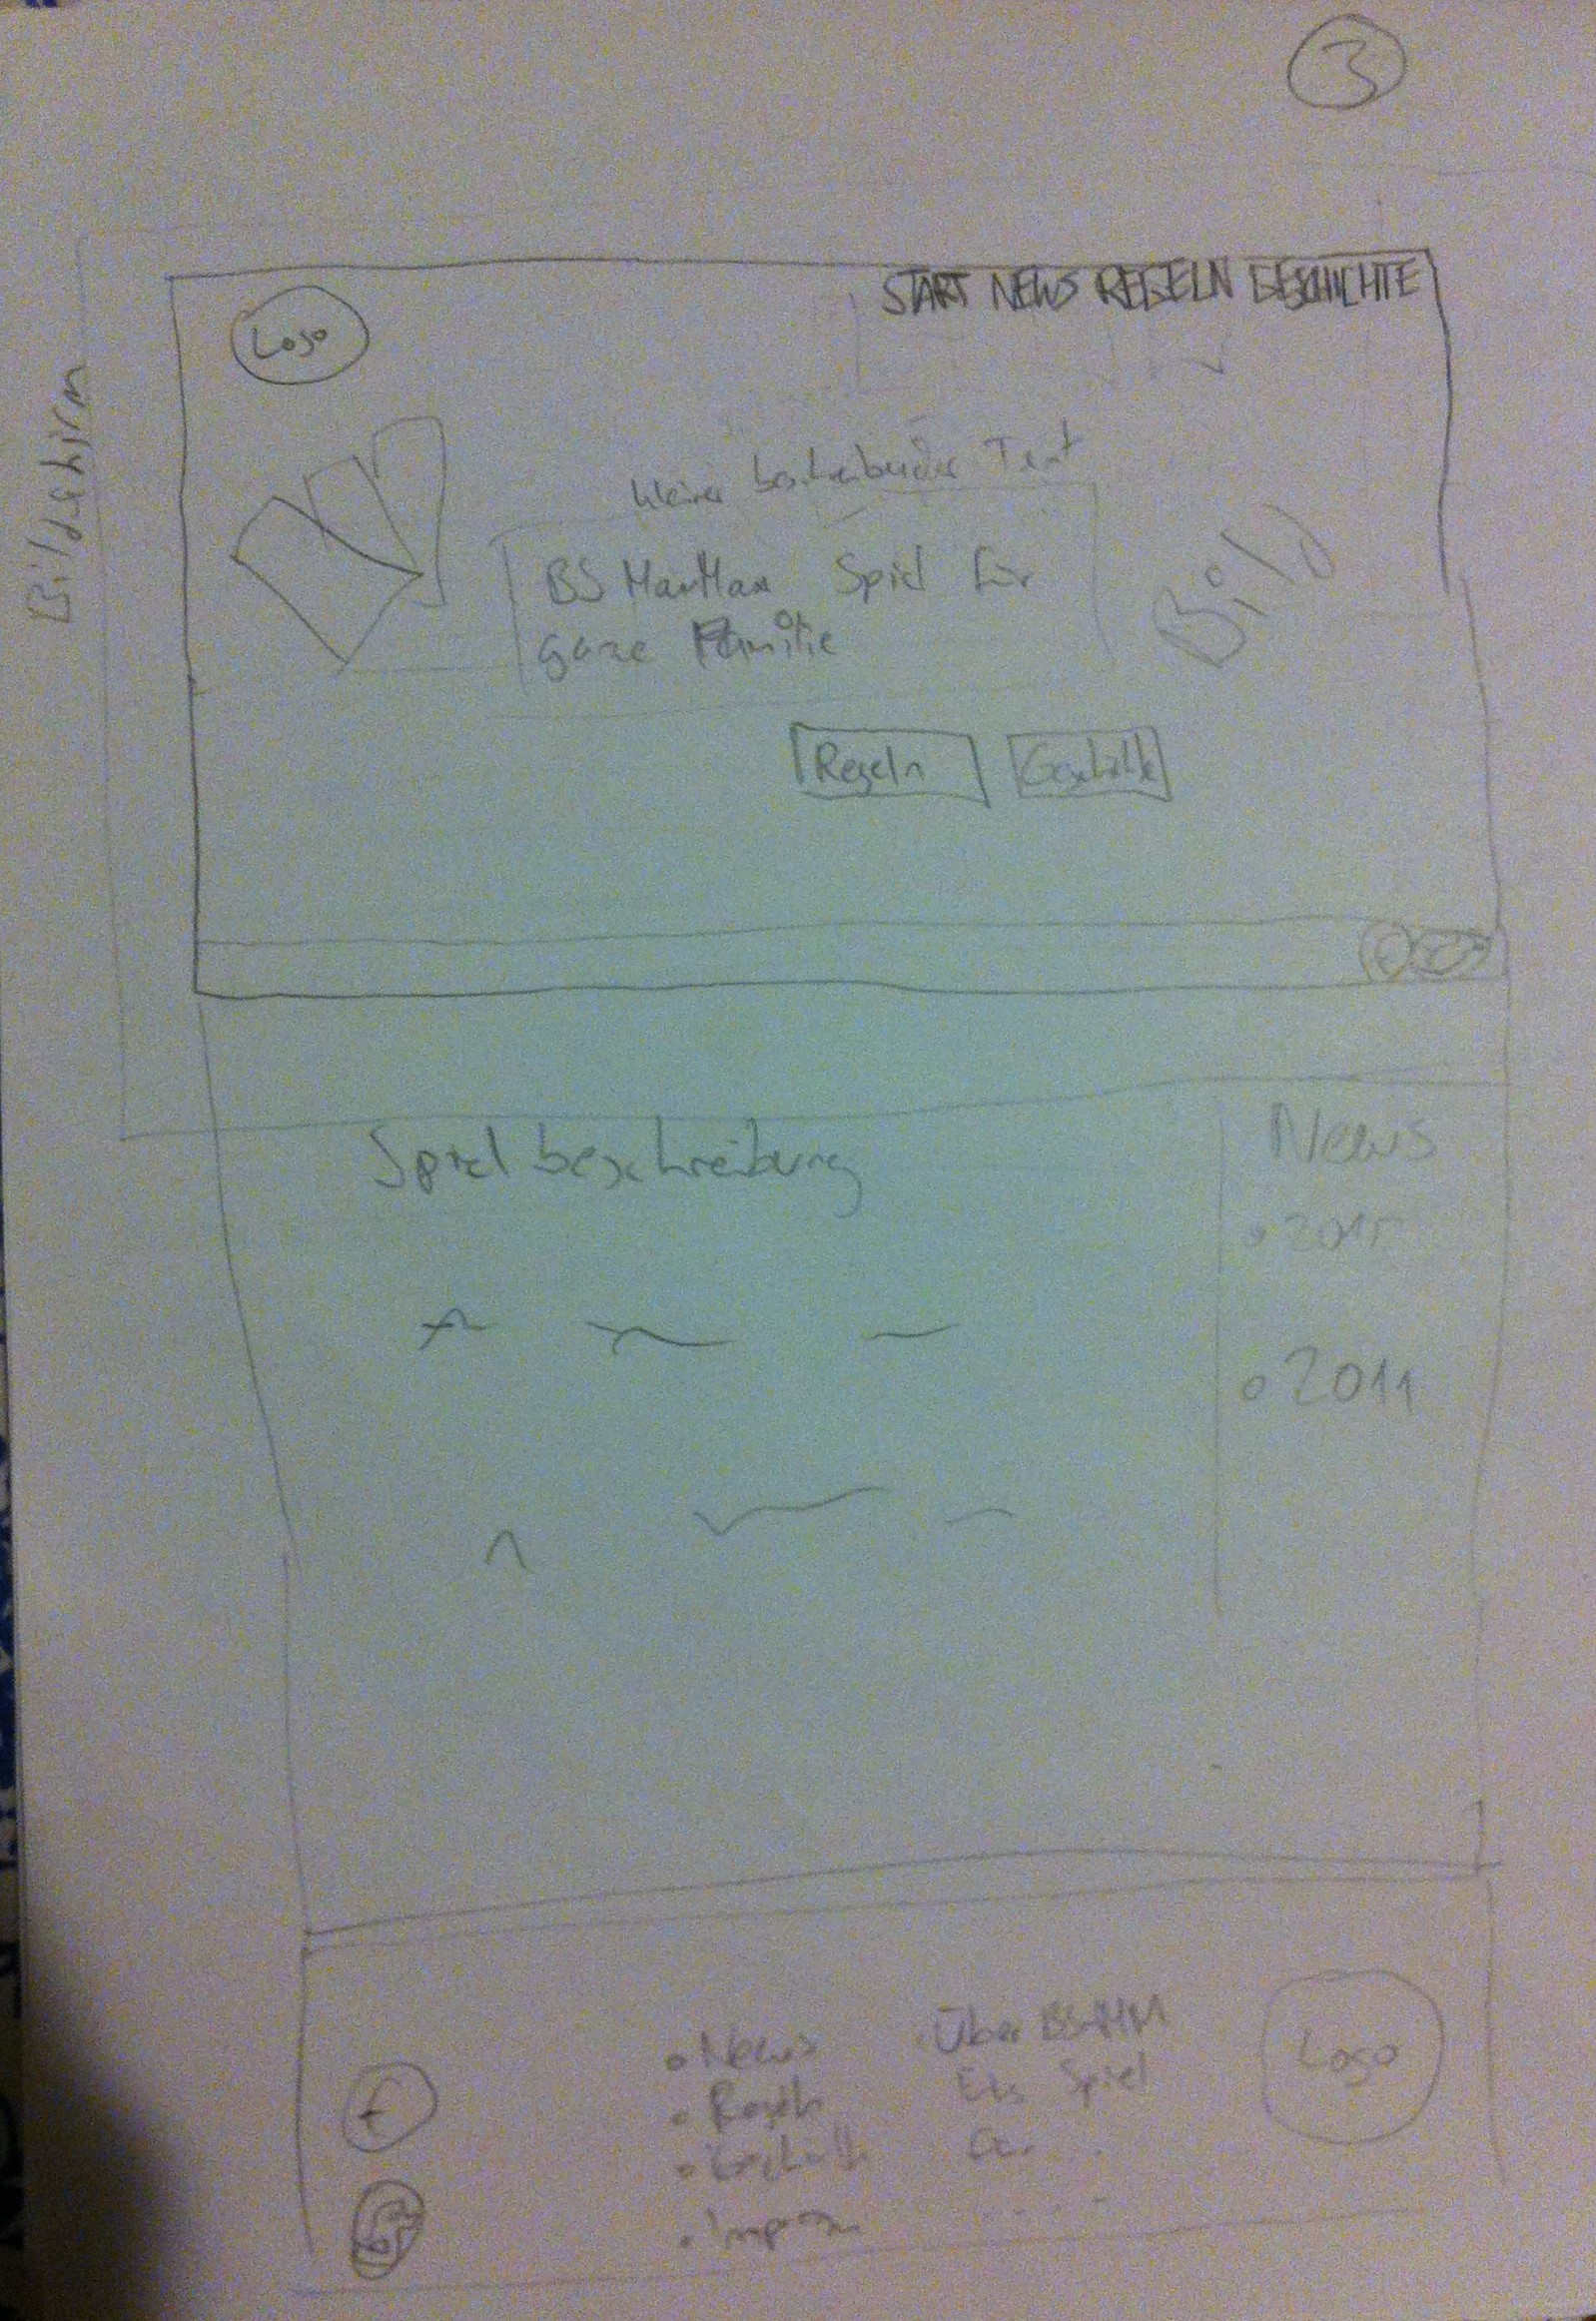
\includegraphics[width=0.7\textwidth]{Version3.jpg}
\caption{Entwurf 3, Marc}
\end{figure}
 \begin{description}
 \item[Vorteile:] Modernes Design, hat einen "Call-To-Action", der den Nutzer anregt die Seite tiefer zu erkunden
 \item[Nachteile:] Header zu dominant
  \end{description}

 
 \subsection*{4. Entwurf}
   \begin{figure}[H]
 \centering
   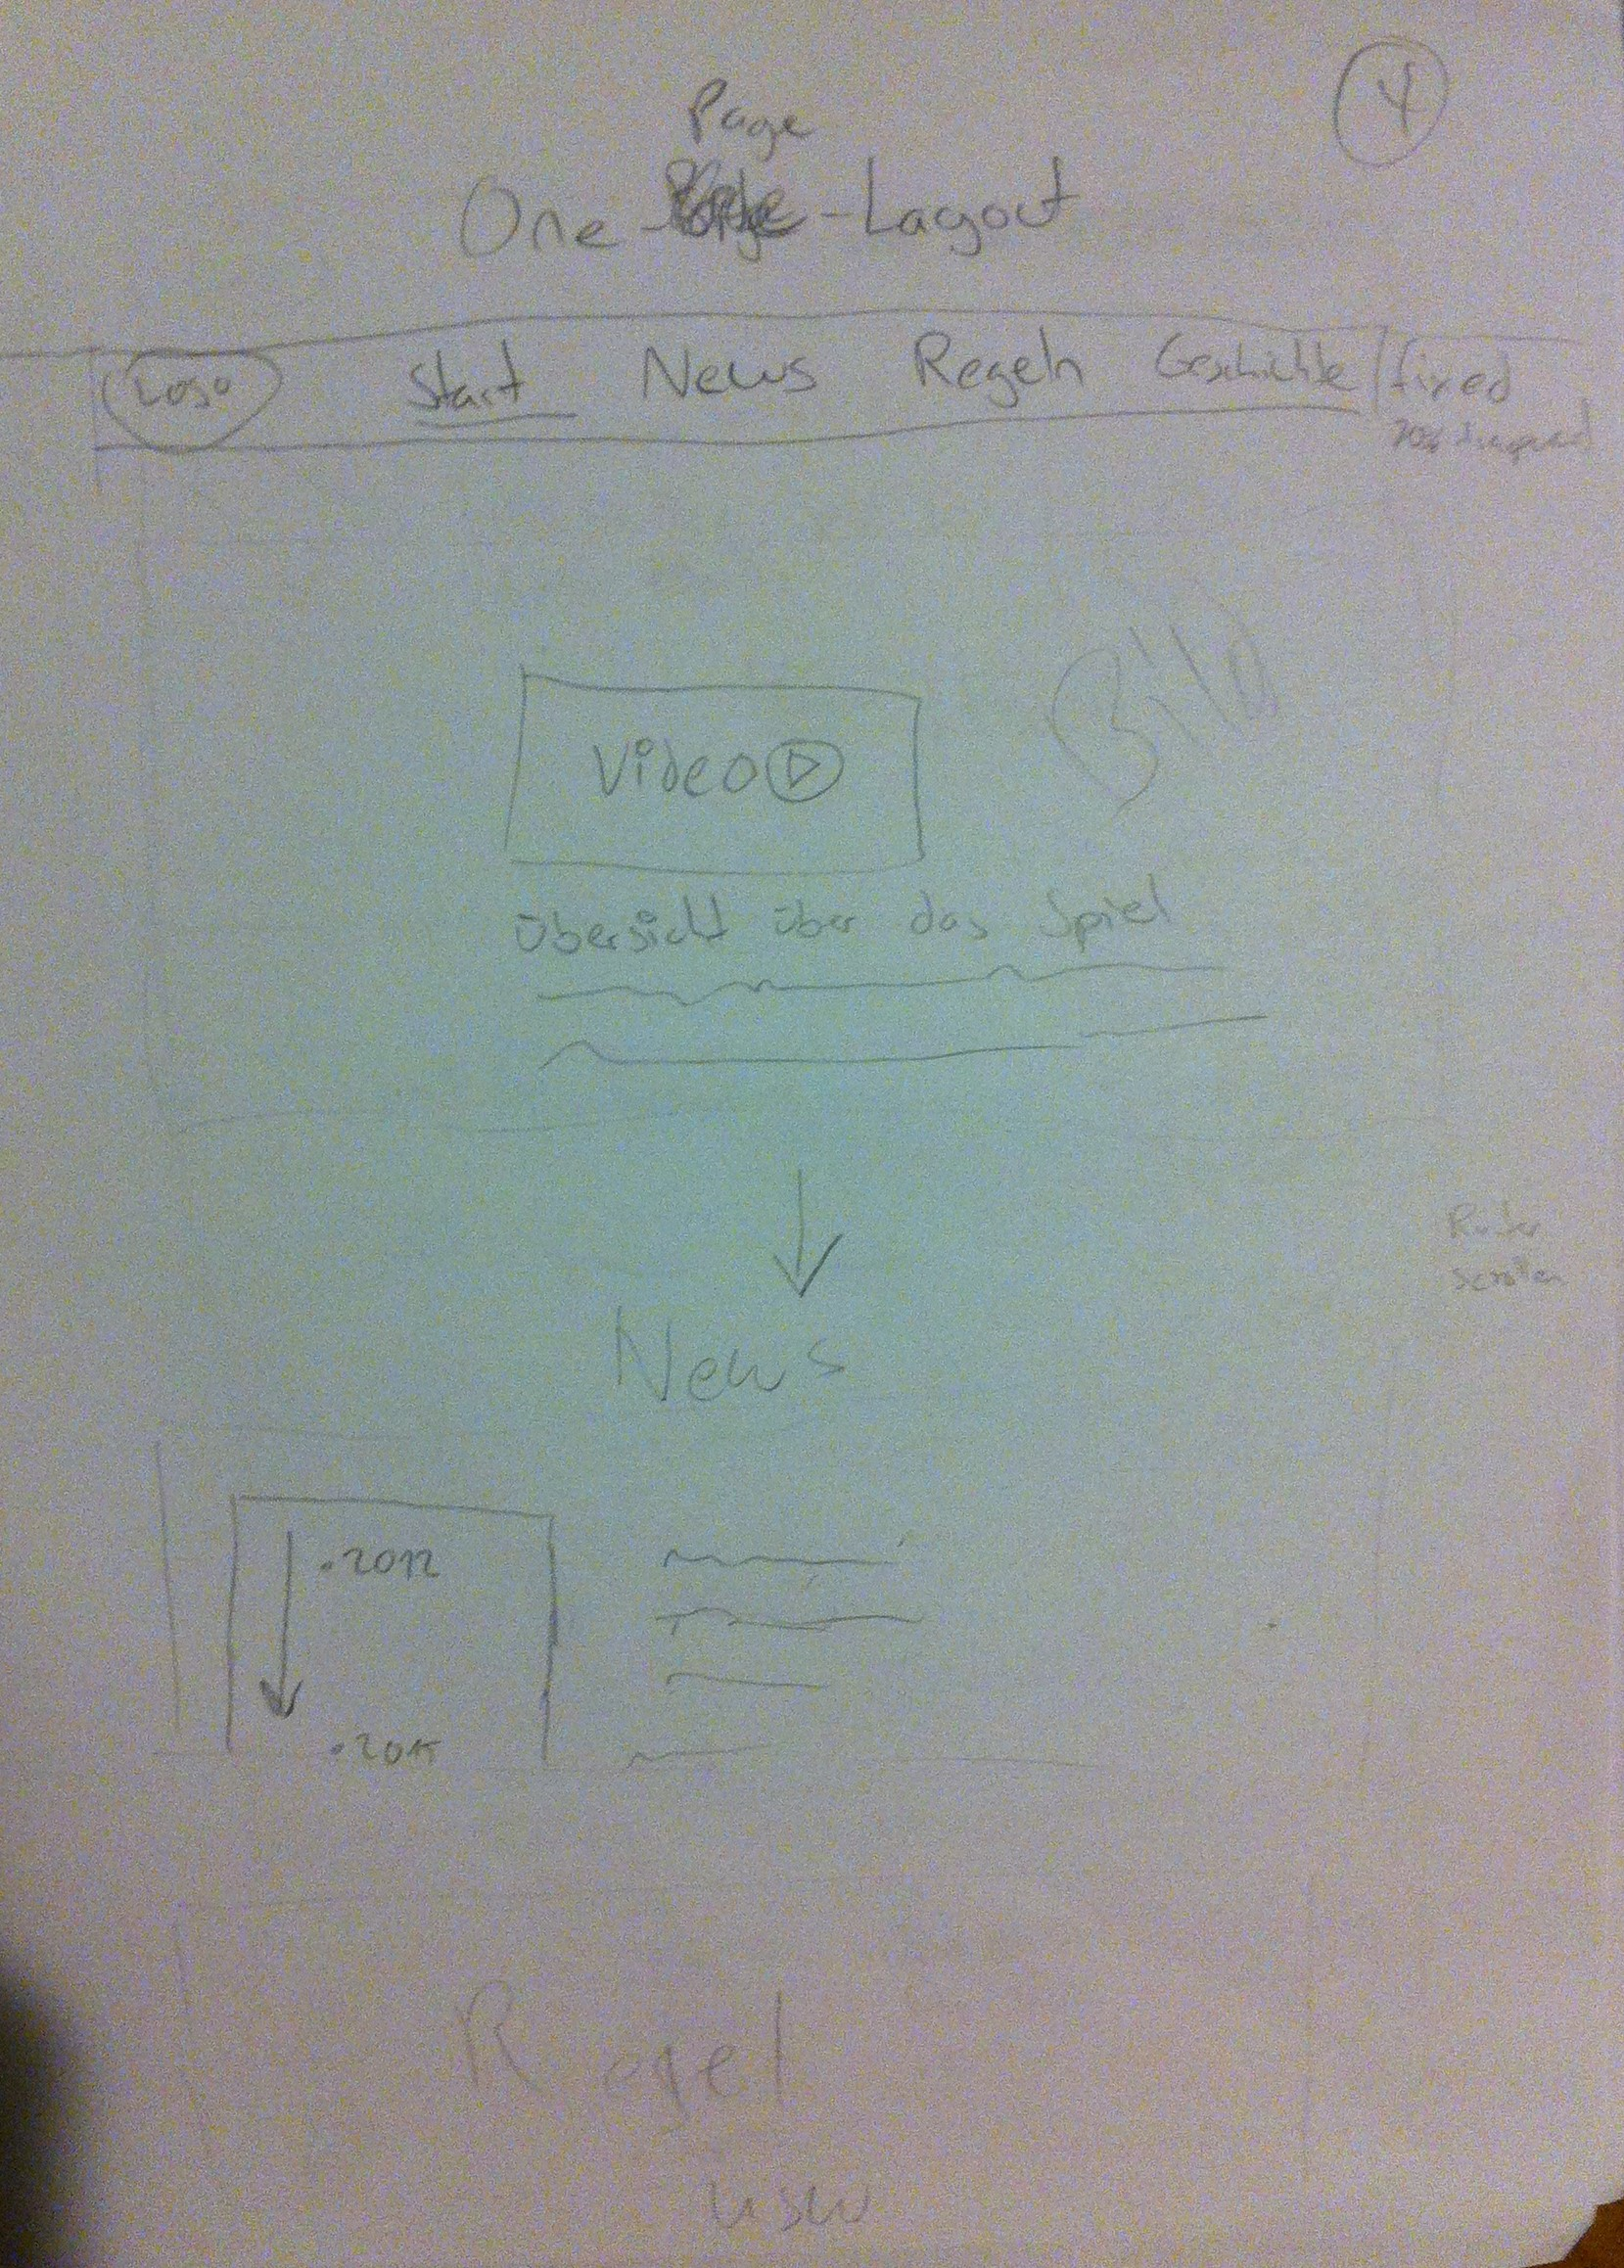
\includegraphics[width=0.7\textwidth]{Version4.jpg}
\caption{Entwurf 4, Marc}
\end{figure}

 \begin{description}
 \item[Vorteile:] Video: Manche Nutzer schauen lieber Videos, als Text zu lesen, Aktuelles Design, Visuell anprechendes Design
 \item[Nachteile:] Video: Manche Nutzer könnten sich dadurch gestört fühlen, lange Ladezeit durch Videodatei, unübersichtlich, da sich der gesamte Inhalt auf einer Seite befindet und gescrolled werden muss, um alles zu erreichen. Der Nutzer benötigt so möglicherweise mehr Zeit, um bestimmte Informationen zu finden. 
 \end{description}

 
\subsection*{5. Entwurf}
 \begin{figure}[H]
 \centering
   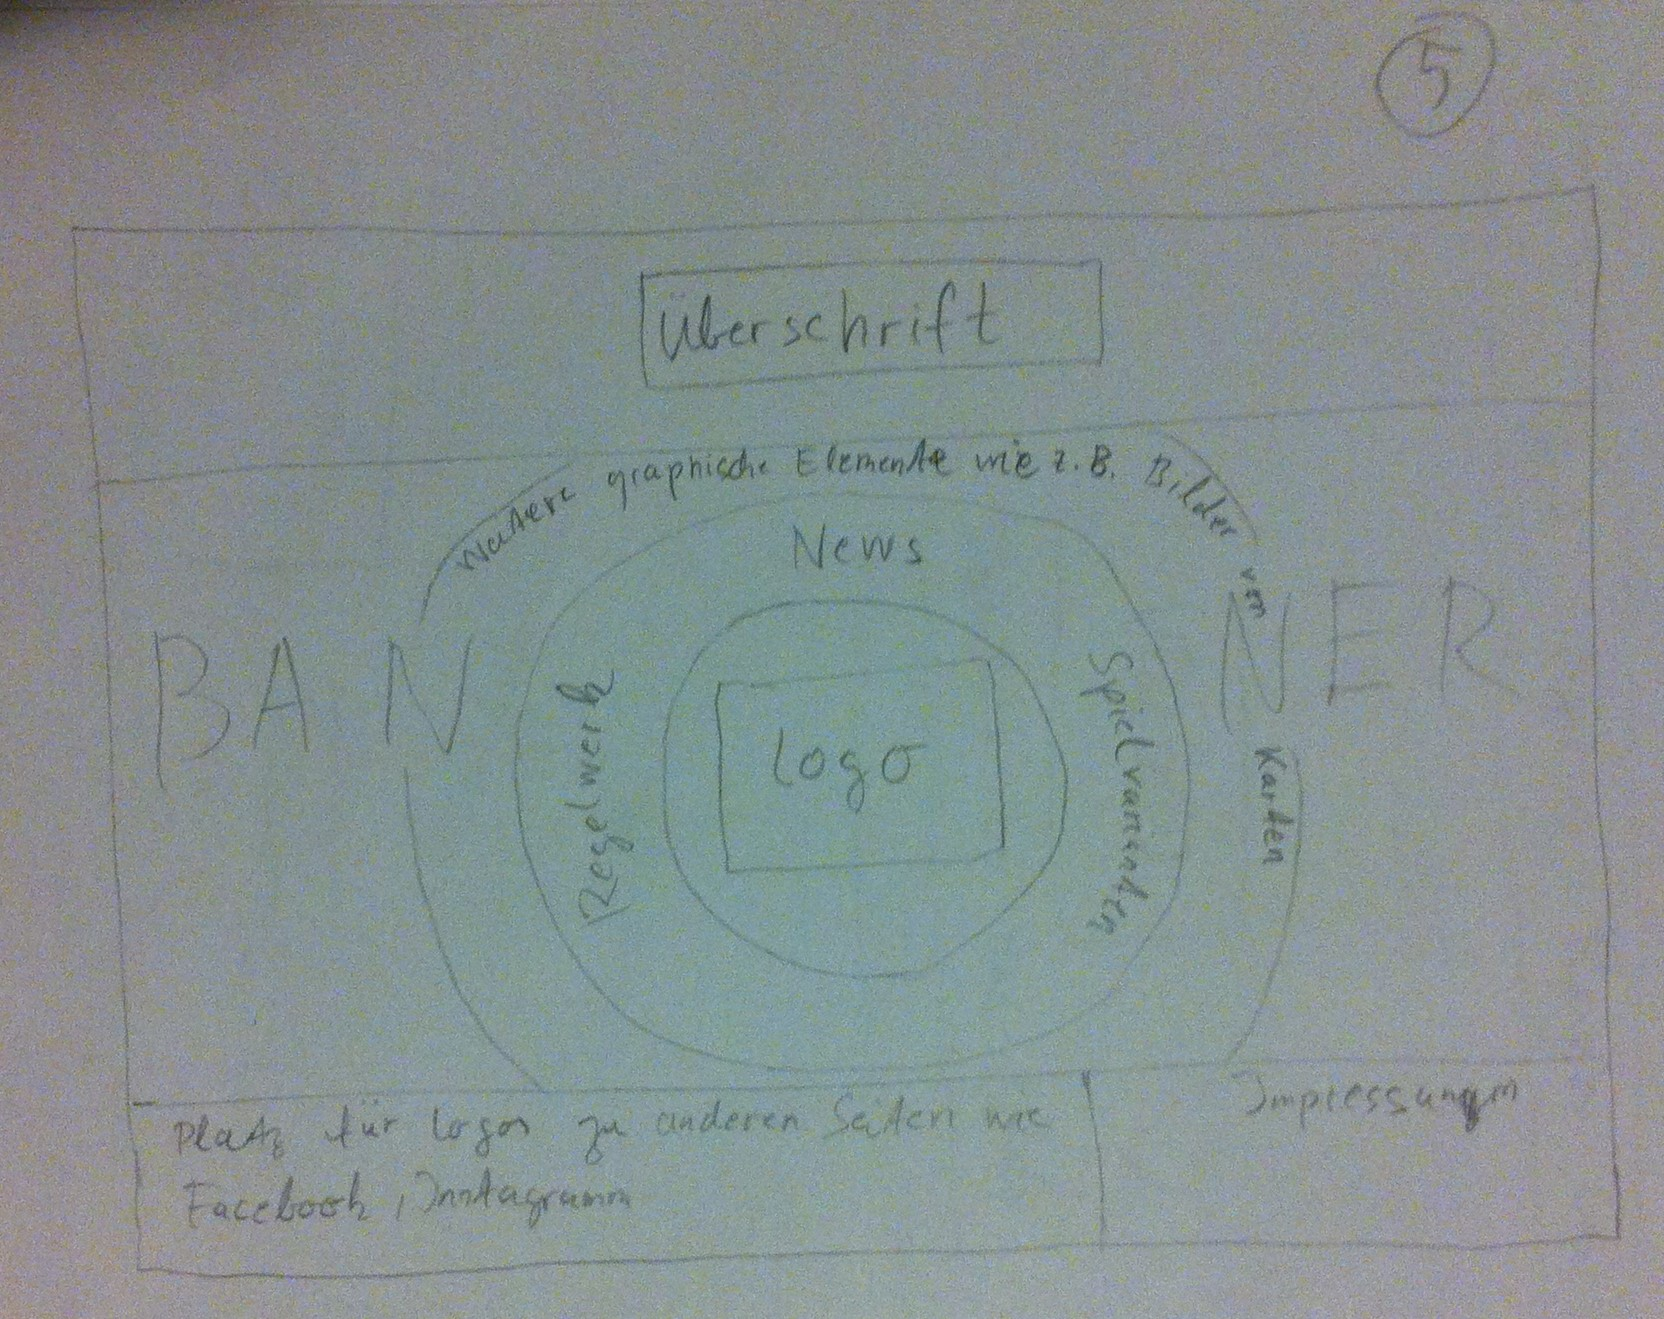
\includegraphics[width=0.7\textwidth]{Version5.jpg}
\caption{Entwurf 5, Ulli}
\end{figure}
 \begin{description}
 \item[Vorteile:]Aufwändiges, spezielles, daher einprägsames Design
 \item[Nachteile:] Hoher Programmieraufwand, möglicherweise zu kompliziertes Design für Nutzer, bedingt smartphonetauglich, bräuchte noch eine Übersicht für Erstnutzer
 \end{description}
 
\subsection*{6. Entwurf}
 \begin{figure}[H]
 \centering
   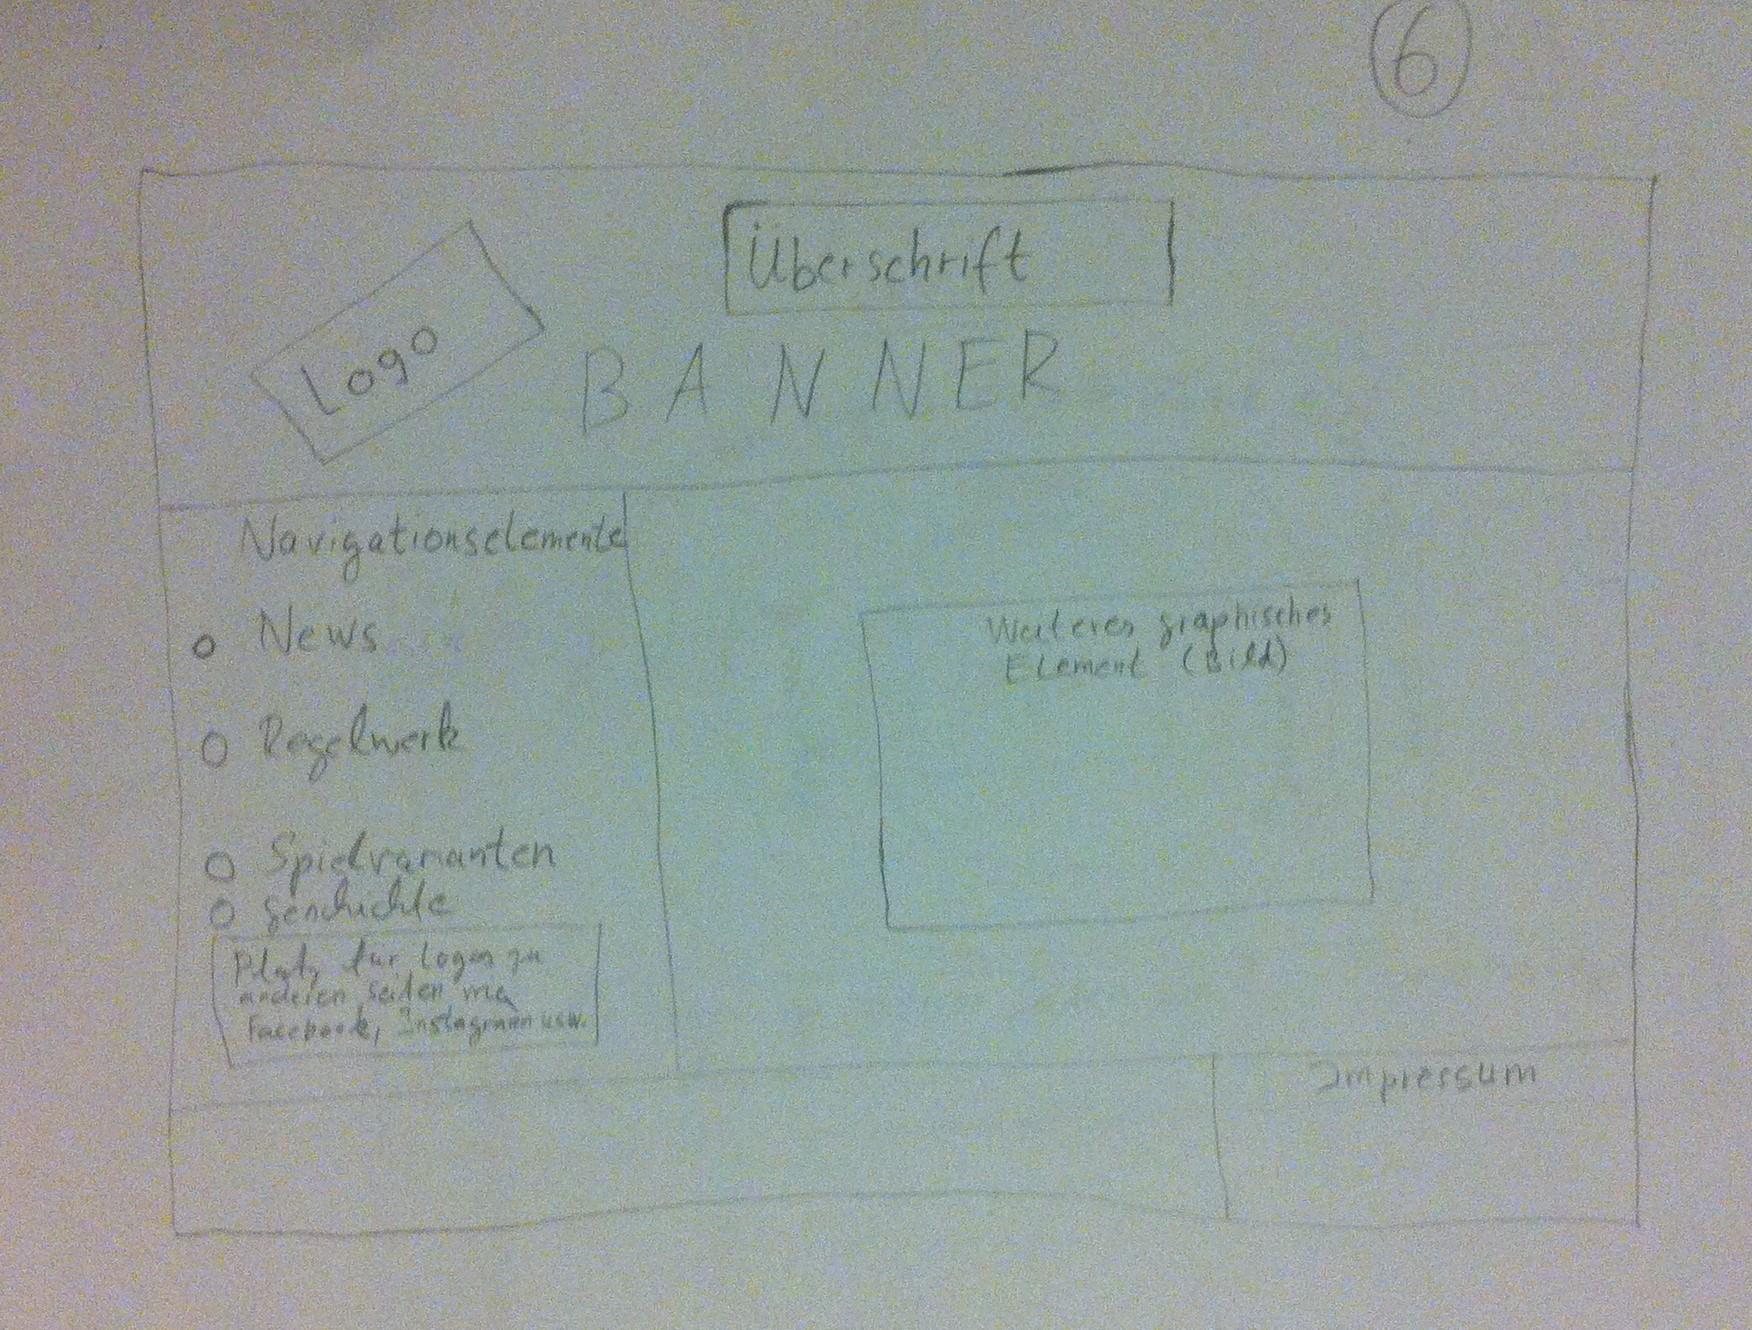
\includegraphics[width=0.7\textwidth]{Version6.jpg}
\caption{Entwurf 6, Ulli}
\end{figure}
 \begin{description}
 \item[Vorteile:]  Einfache Struktur, übersichtlich, benutzerfreundlich, dynamisches Design durch schräges Logo, Bilder statt Text kann interessanter wirken 
 \item[Nachteile:] Nicht besonders anprechend, veraltetes Design bezüglich der Navigationsleiste
 \end{description}

\subsection*{Ergebnisse}
 Wir wollen eine feste Navigationszeile, die auf jeder Seite gleich ist. Nur der Titel der momentan geöffneten Seite soll markiert werden.
 Als Hintergrundbild der Navigation stellen wir uns ein Bodenseebild oder Spielkarten vor. \\
 \\ 
 Die \textit{Startseite} (index.html) bekommt einen Call-To-Action, der anregt auf die Unterseite \textit{Regeln} oder \textit{Geschichte} zu gehen. Unter dem Call-To-Action gibt es einen kurzen beschreibenden Text über das Spiel (interessant für Erstnutzer). \\ \\
Die \textit{Regeln}-Seite bekommt zusätzlich zur oberen Navigation, eine linke feste Navigation. 
   \\  \\
  Das \textit{Impressum} soll nur ein einfacher, linksbündiger Standarttext werden.
\section*{Aufgabe 4: Papierprototyp erstellen}
Der feste Teil des Papierprototypen ist die Webseite, welche von einem Browser-Rahmen (Größe DINA-3) umrahmt wird. Der obere Teil der Webseite zeigt einen fixierten Header, zu dessen Repräsentation ein farbiger Streifen verwendet wurde, welcher auf den Hintergrund aufgeklebt wurde. Später soll er aus einem Bild bestehen, z. B. Karten oder ein Bild vom Bodensee. Um später die \textit{Scrollbarkeit} der Webseite darstellen zu können, wurde jedoch ein Schlitz in den Rahmen hinter dem Header gemacht, wodurch die Seite bei der Demonstration des Runter- bzw. Hochcrollens einfach durchgezogen werden kann. Ein kleiner Pfeil, der mit einer Büroklammer am Header befestigt ist, kann verschoben werden und dazu genutzt werden, anzuzeigen, auf welcher Seite sich der Besucher der Seite gerade befindet. Der Footer ist im Gegensatz zum Header nicht fixiert, sondern bewegt sich mit dem Inhalt der jeweils ausgewählten Seite. Auf Grund dessen wird er nur mit einer Büroklammer jeweils am unteren Ende der einzelnen Seiten befestigt. Der \glqq Call-to-Action\grqq{} Teil auf der Startseite wurde extra mit farbigem Papier hervorgehoben. Ansonsten sind alle Seiten mit Text als Inhalt mit DINA-4 Blättern dargestellt, so dass links und rechts von ihnen der Hintergrund der Seite zu sehen ist.
Überschriften und Unterüberschriften wurden mit Edding oder Fineliner übertragen. Der Fließtext auf den Seiten wurde mit Wellenlinien symbolisch dargestellt. Die seitlichen Navigationsleisten, welche auf manchen Seiten erscheinen, wurden durch einen extra Papierstreifen dargestellt, da diese teilweise fixiert sind. Als Klebematerial wurde häufig Tesa verwendet um z.B. die Unterseiten teilweise auf zwei Seiten zu verlängern (um auch Scrollen besser darstellen zu können), da manche Seiten länger sind als andere.
  \subsection*{1. Startseite}
 \begin{figure}[H]
 \begin{center}
 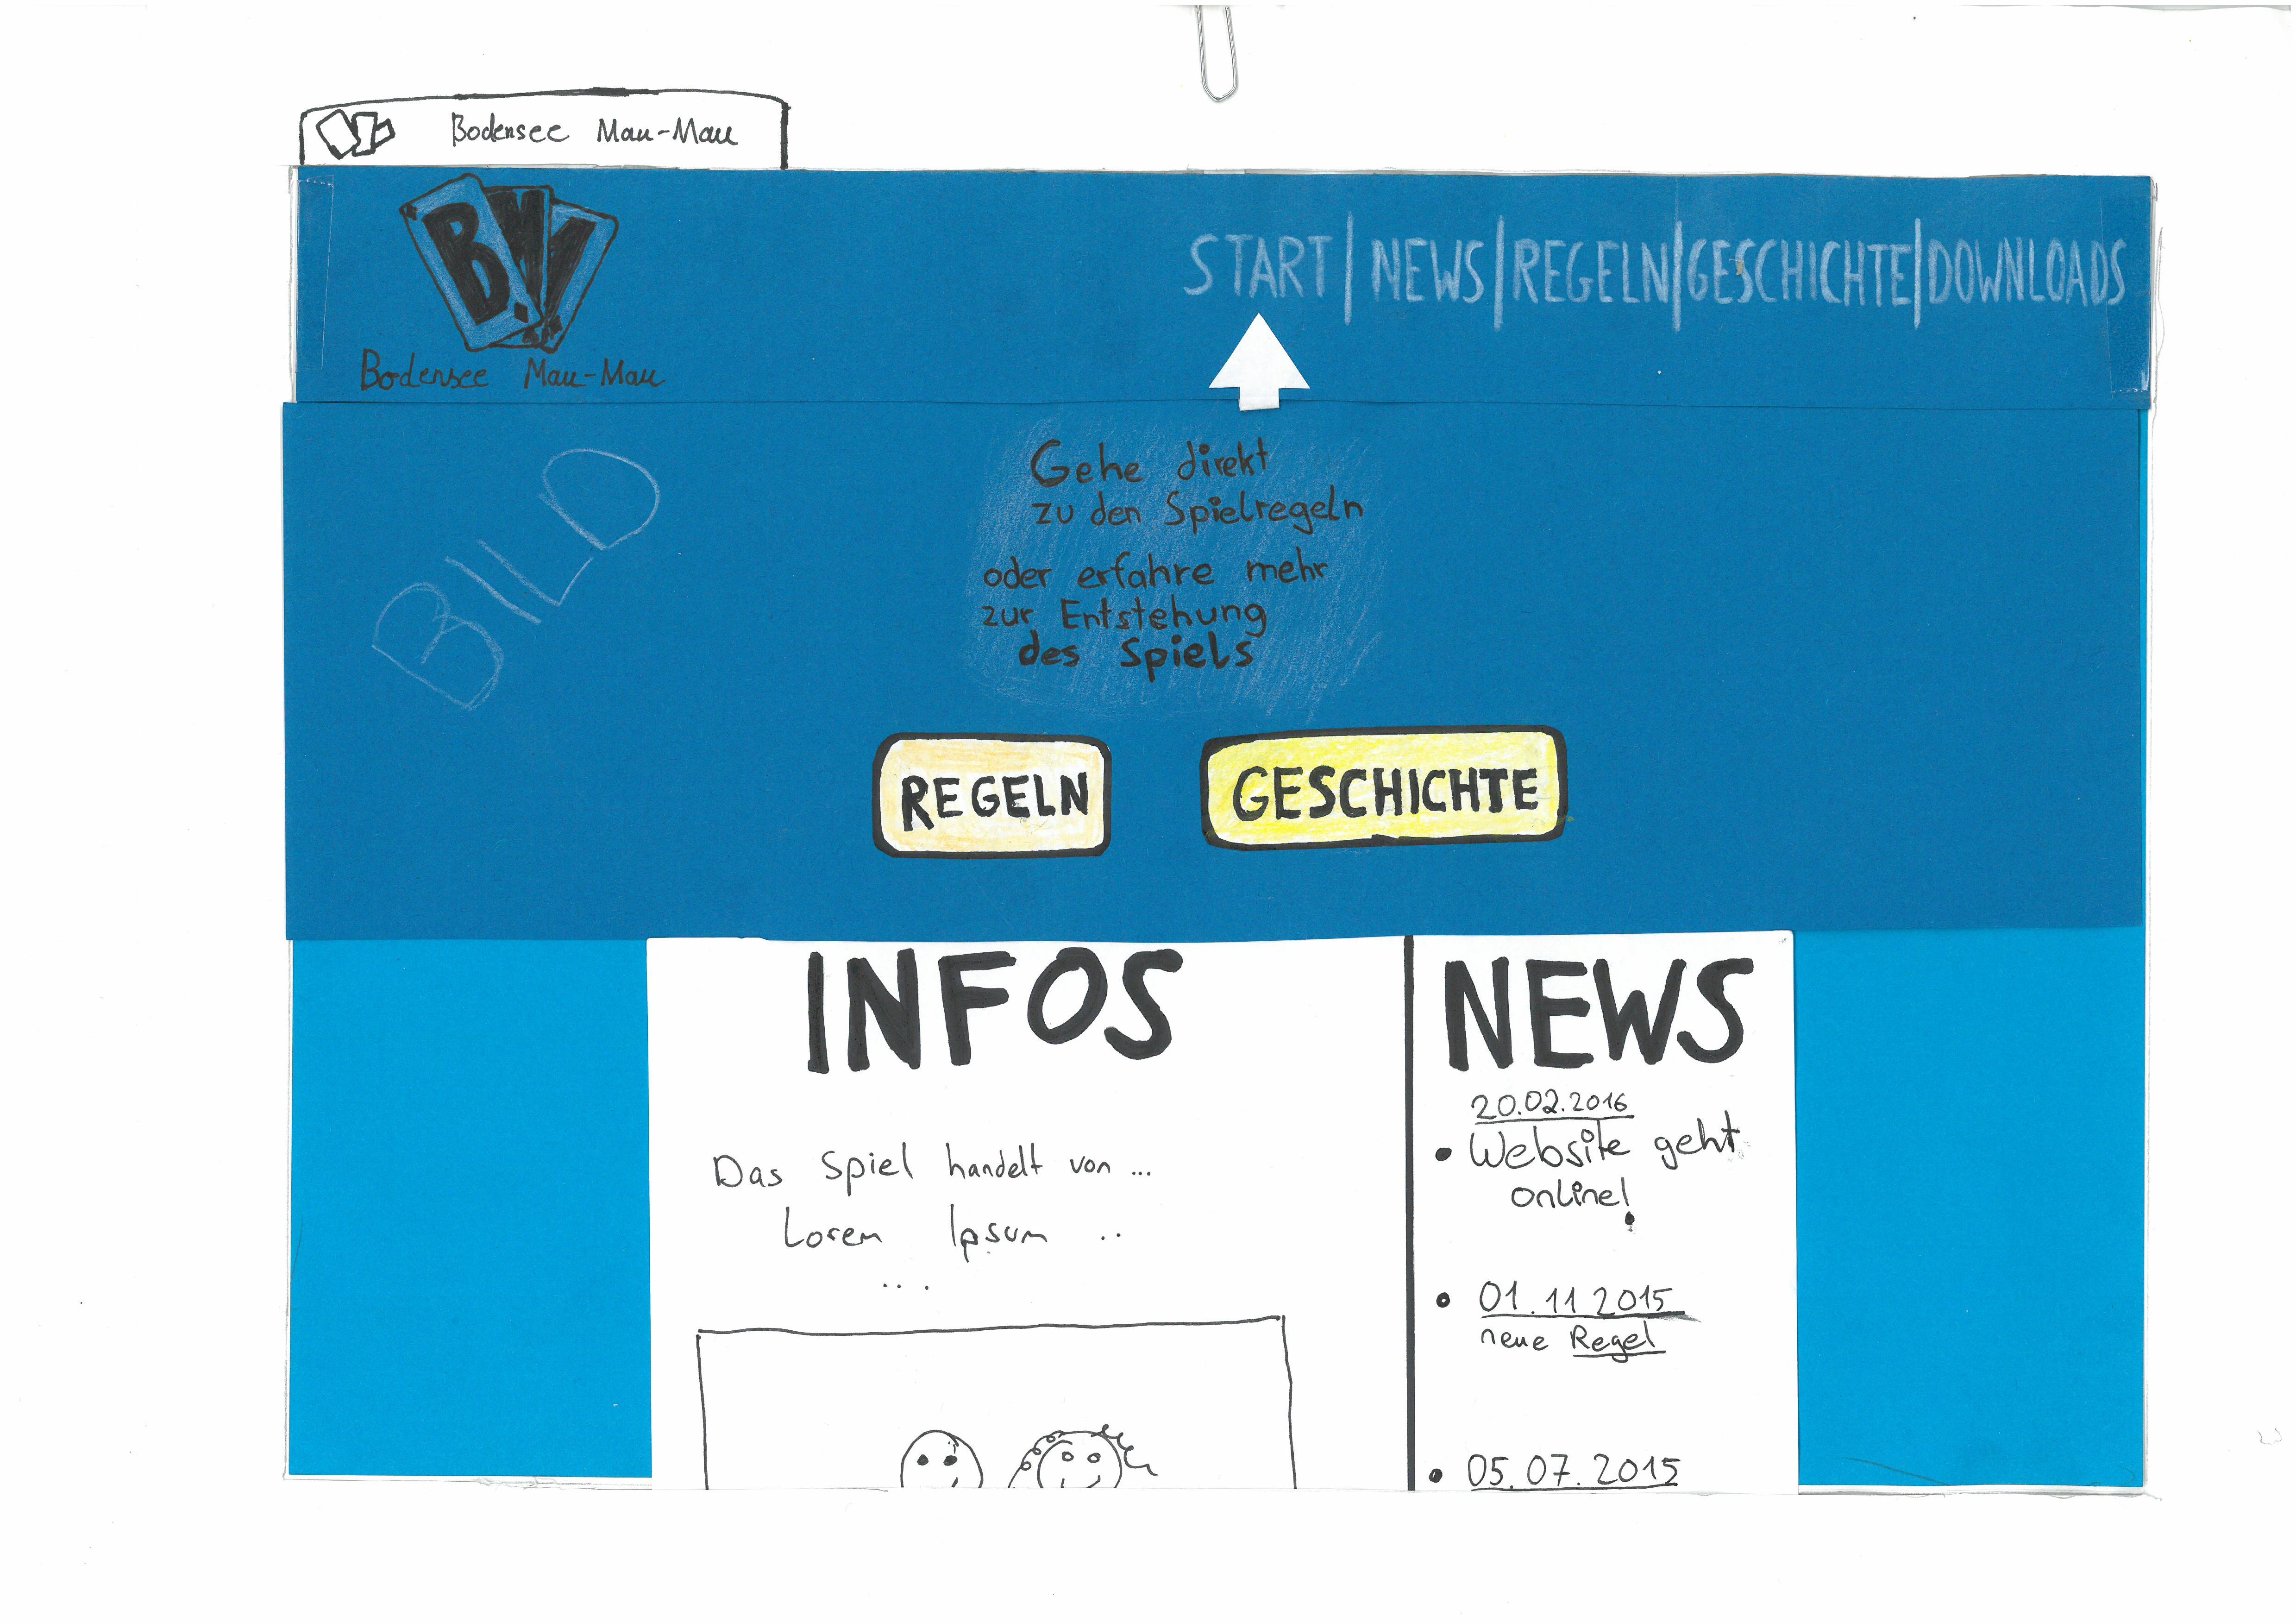
\includegraphics[width=0.9\textwidth]{start-oben.jpg}
\caption{Oberer Teil von index.html}
 \end{center}
\end{figure}
 \begin{figure}[H]
 \begin{center}
 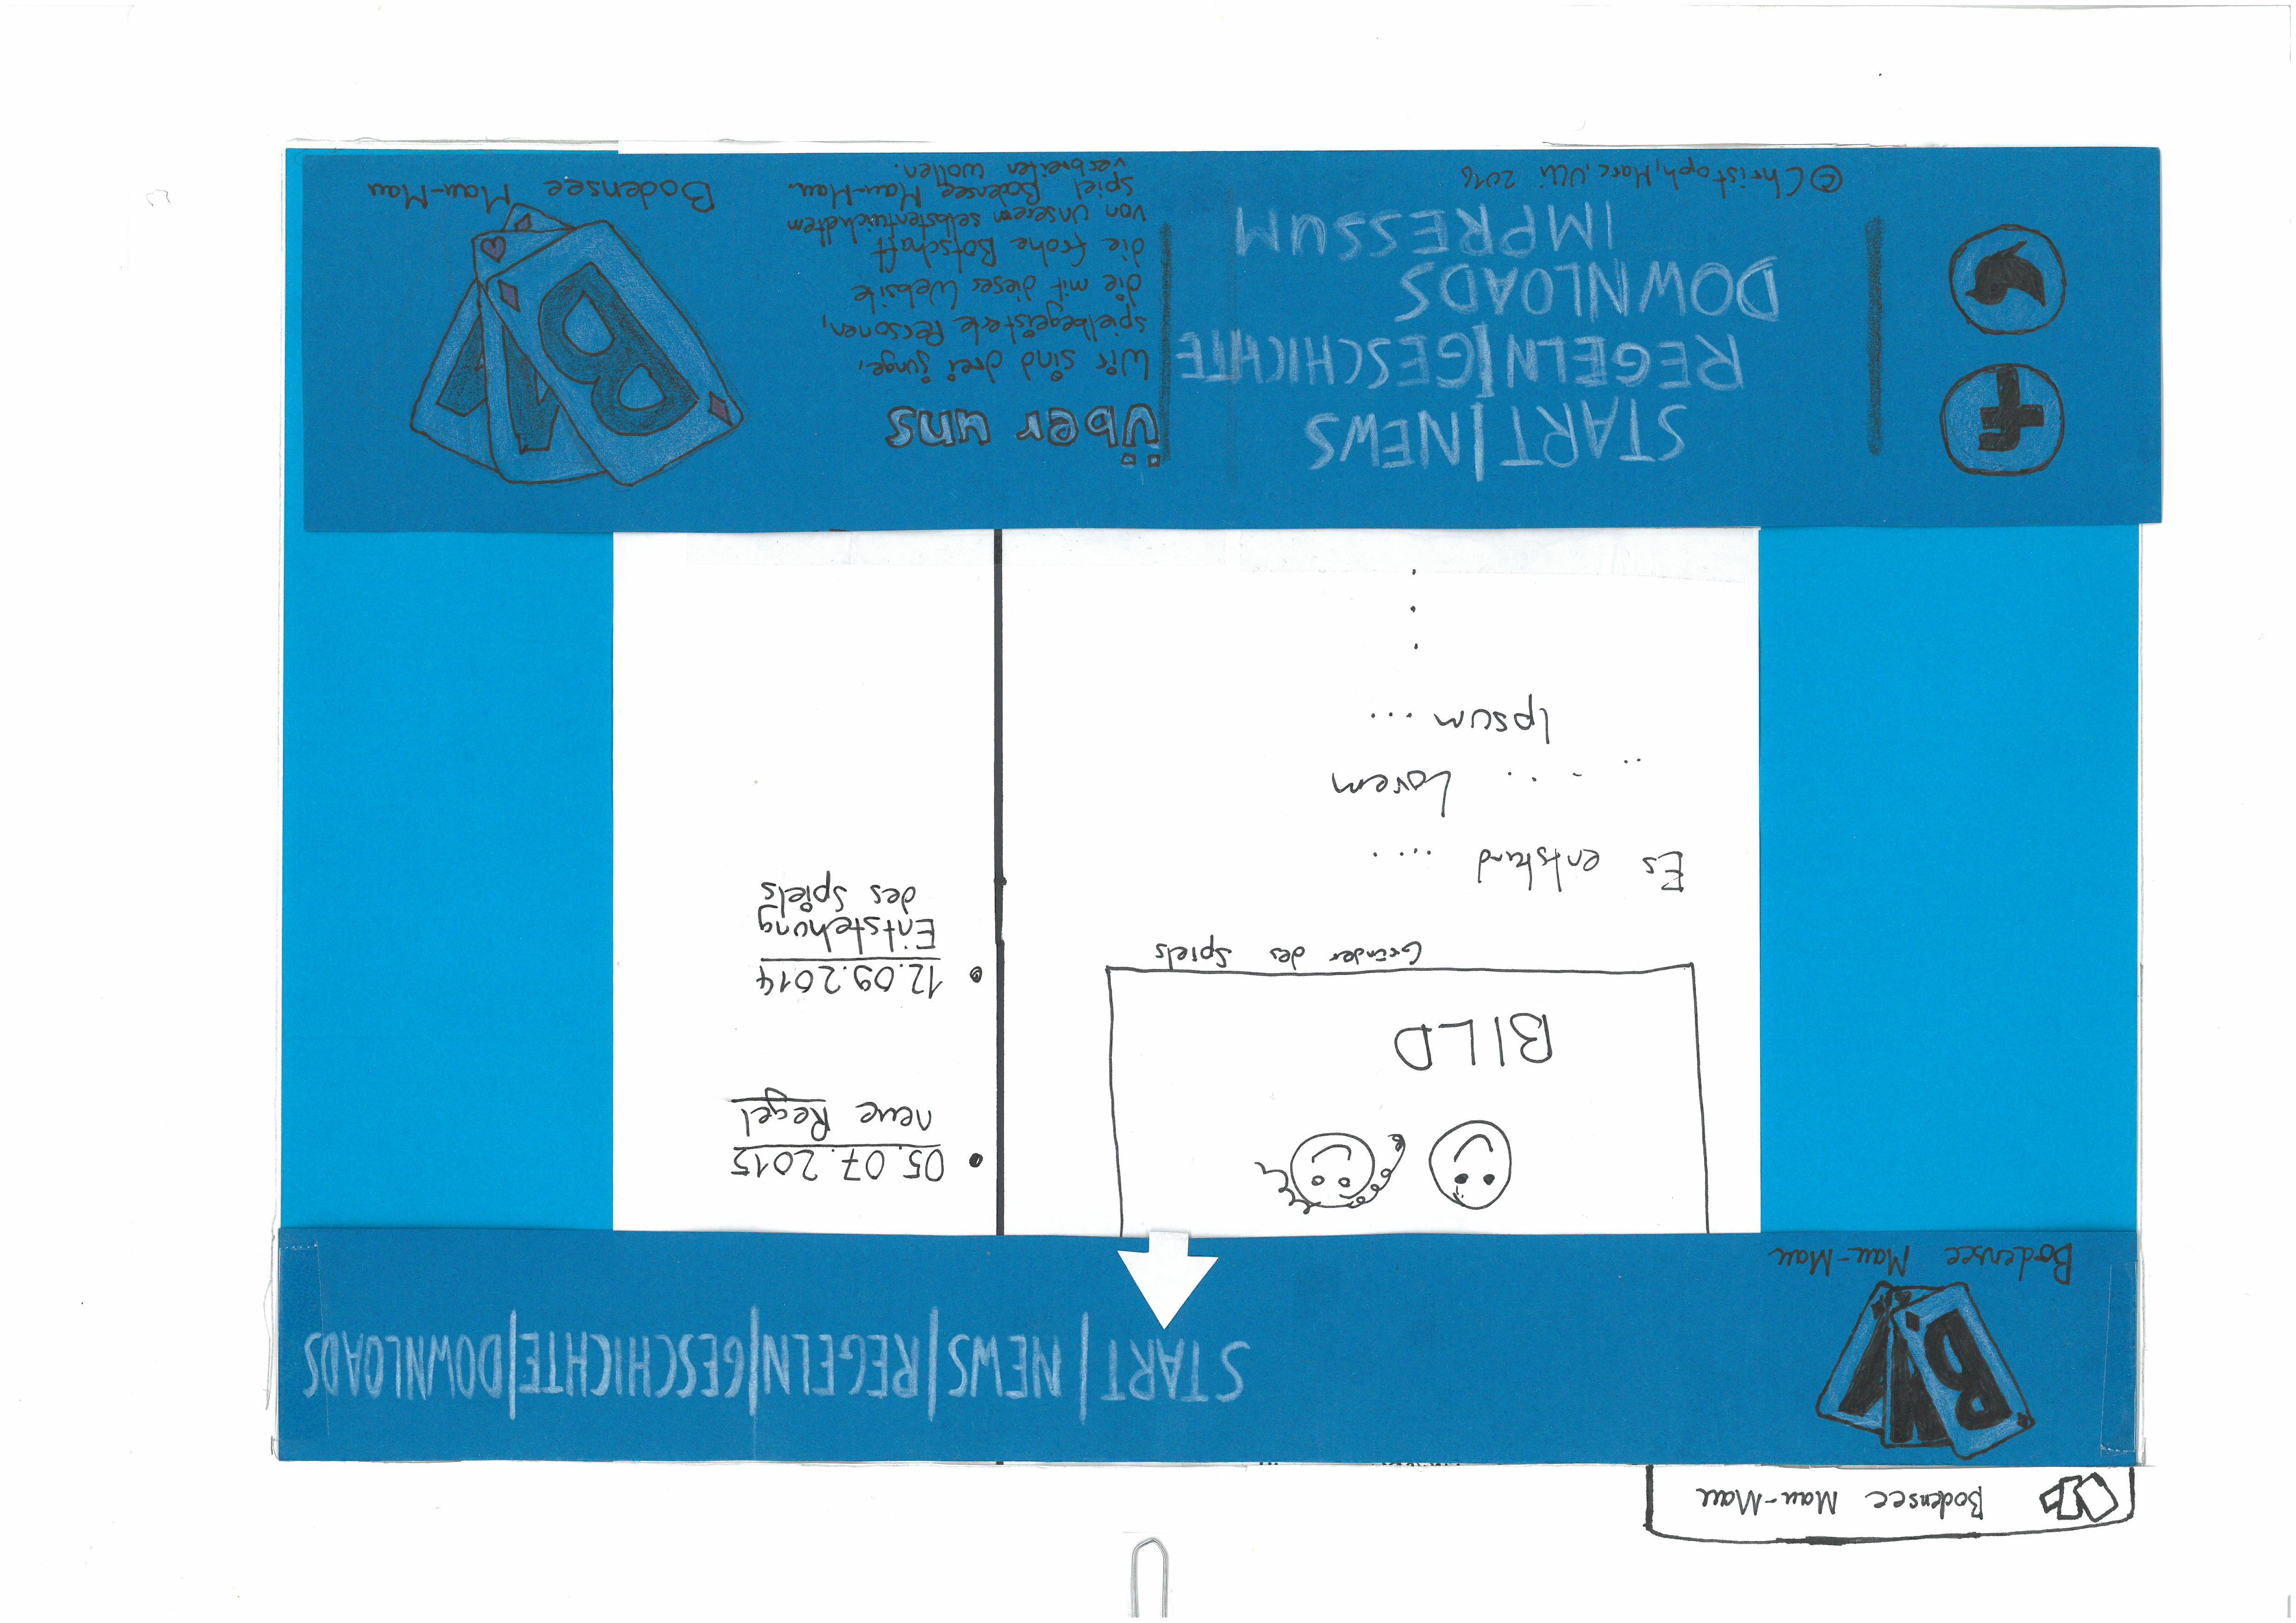
\includegraphics[width=0.9\textwidth, angle = 180, ]{start-unten.jpg}
\caption{Zum Footer runtergescrollt bei index.html}
 \end{center}
\end{figure}
Die \textit{Startseite} (index.html) bekommt einen Call-To-Action, der anregt auf die Unterseite \textit{Regeln} oder \textit{Geschichte} zu gehen. Unter dem Call-To-Action gibt es eine Aufforderung entweder per Button zu den \textit{Regeln} zu springen oder zur \textit{Geschichte}. Der Hintergrund des Call-To-Action soll nahtlos an die feste Navigation anknüpfen, doch beim runterscrollen hinter dieser verschwinden. Der restliche Content ist zwei-geteilt. Einerseits (links) in eine längere Beschreibung des Spiels und rechts, durch einen Trennstrich geteilt, Überschriften aus dem Newsbereich. 
  Darunter der Footer. Auf der linken Seite Socialmedia, untereinander angeordnet. Dann die Navigation als Liste, daneben eine kurze Beschreibung des Spiels. Ganz rechts wieder das Logo, diesmal größer dargestellt. Der Footer ist, wie schon erwähnt, auf jeder Seite gleich. 
  \subsection*{2. News}
  \begin{figure}[H]
 \begin{center}
 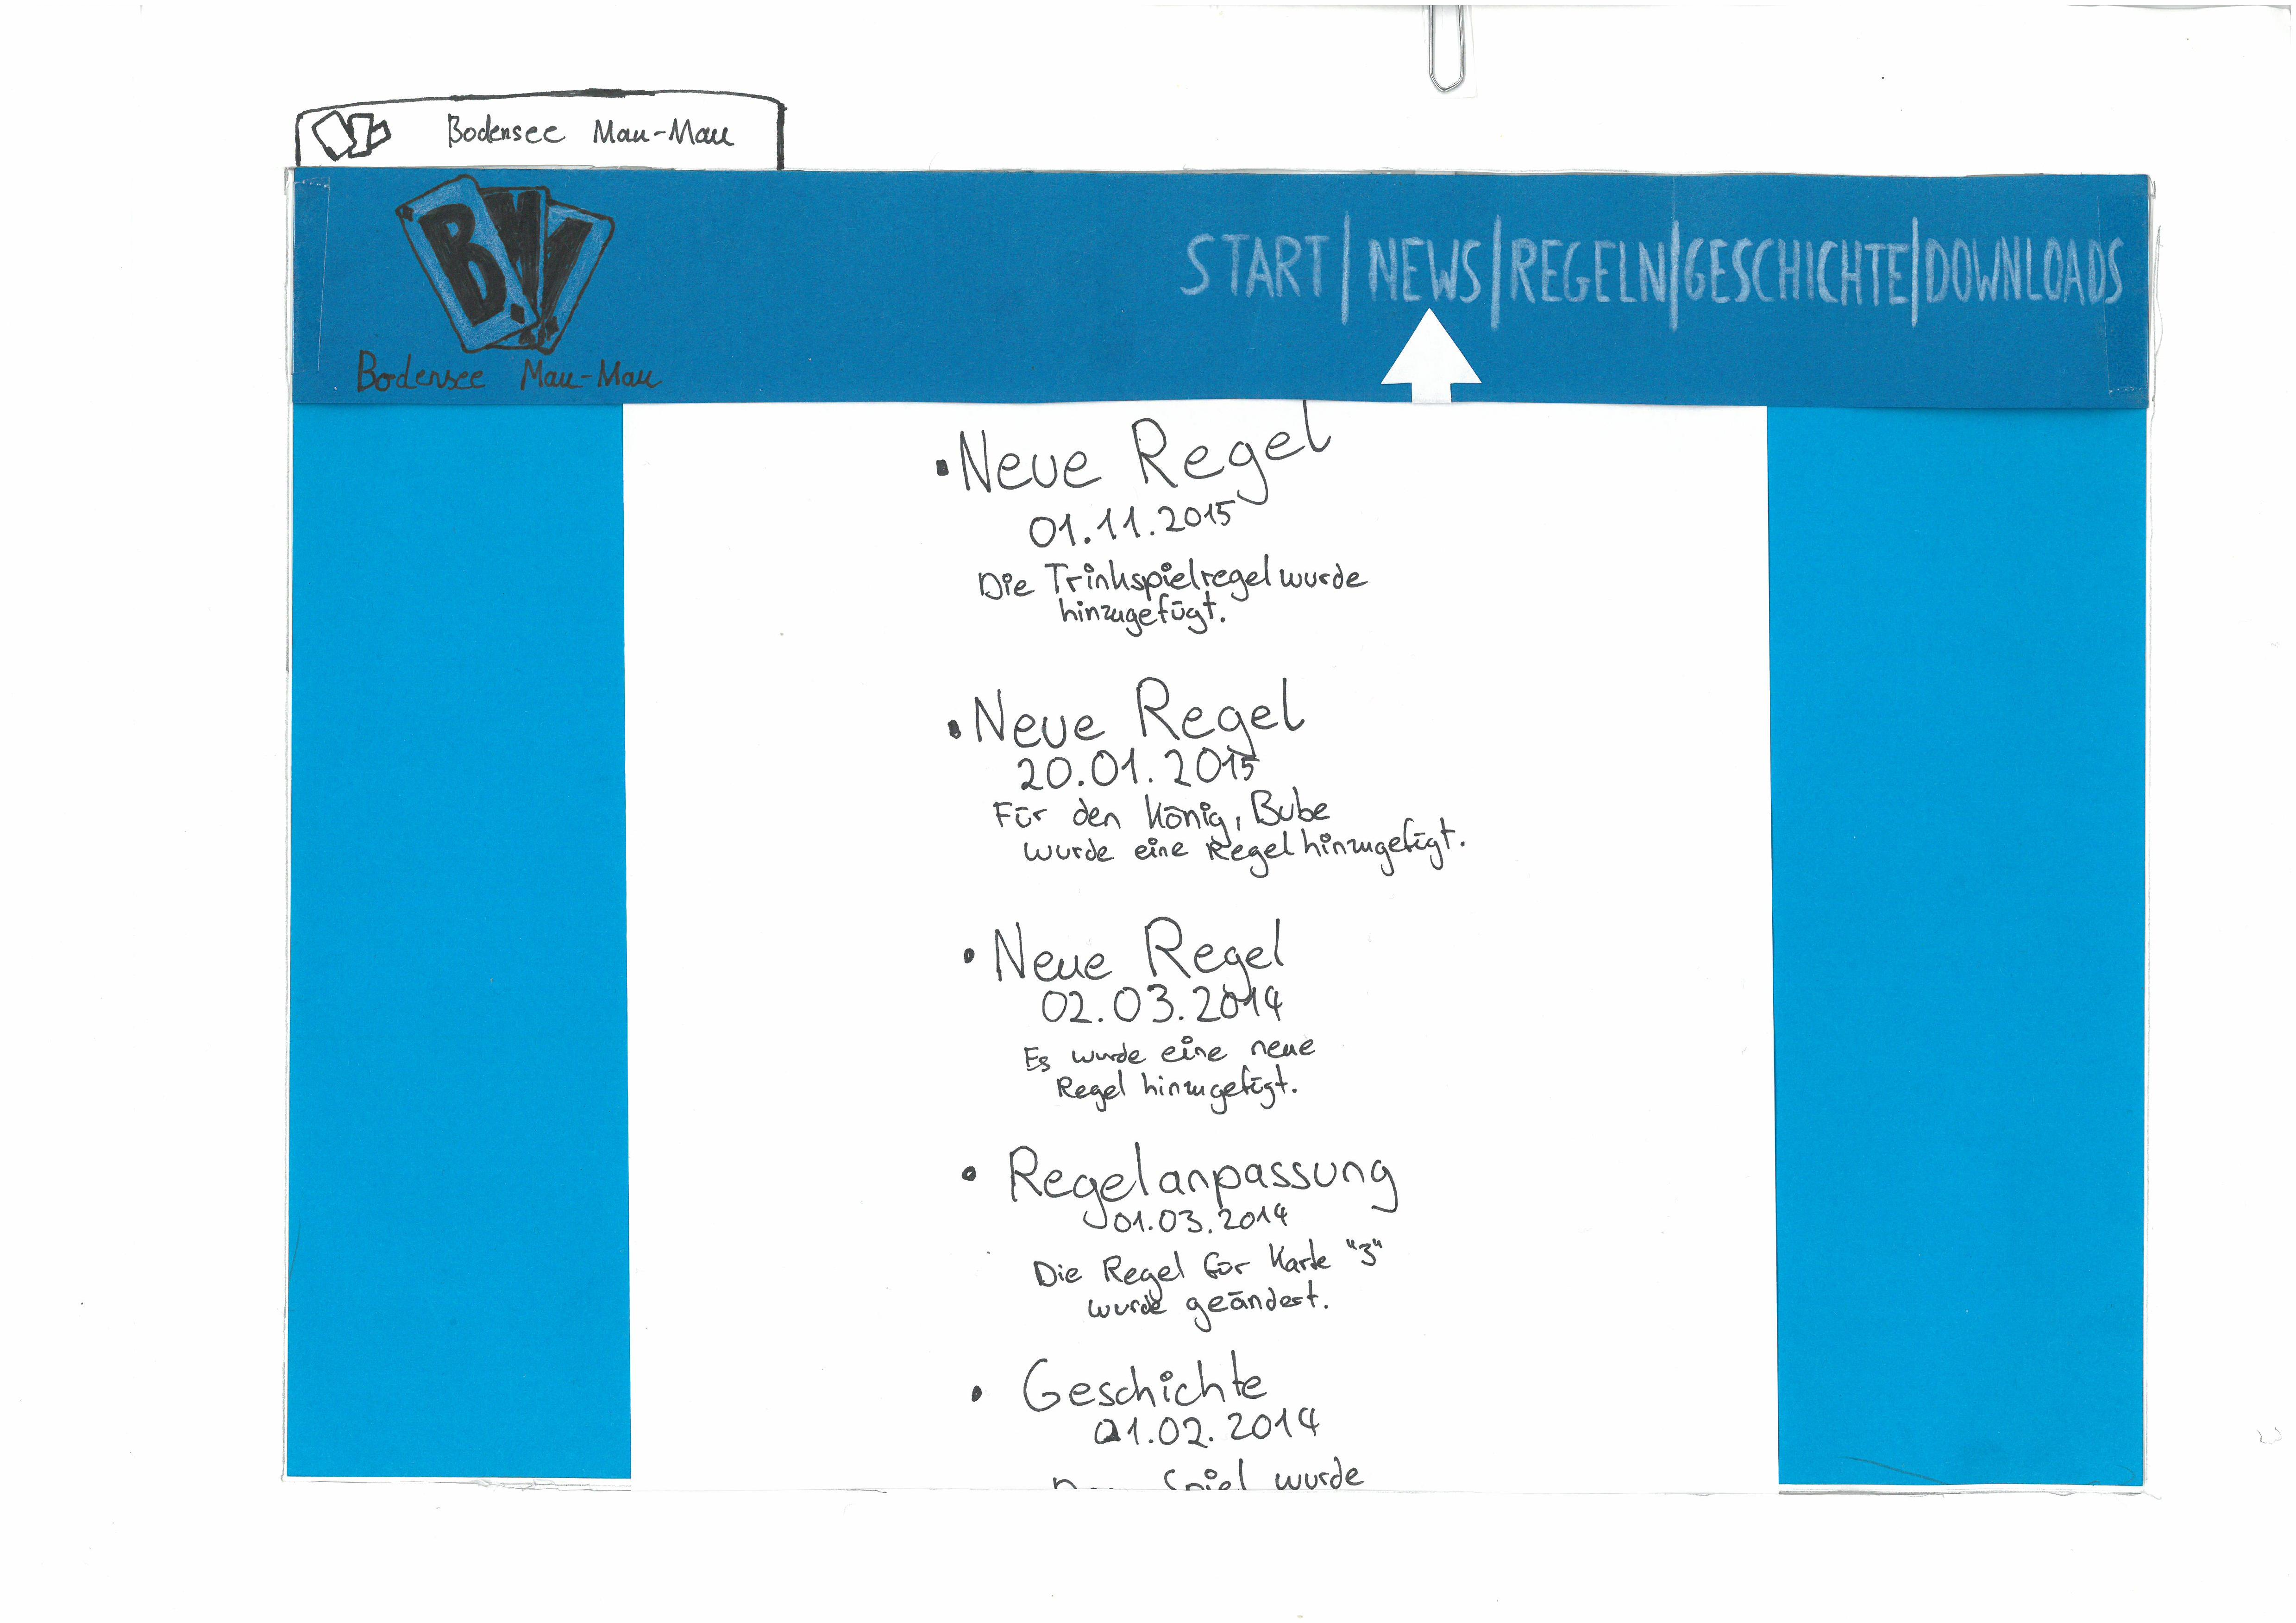
\includegraphics[width=0.9\textwidth]{news.jpg}
\caption{news.html}
 \end{center}
\end{figure}  
  Die \textit{News} sollen zentriert dargestellt werden. Mit dem Datum und Stichwort als Überschrift wird hier kurz gezeigt, was es neues gibt. Gestartet wird mit dem aktuellstem Content (oberster Eintrag). Sind neue Regeln entstanden, sind diese verlinkt, zur Seite \textit{Regeln}, an die Stelle wo sie eingefügt wurden.
  \subsection*{3. Regeln}
  \begin{figure}[H]
 \begin{center}
 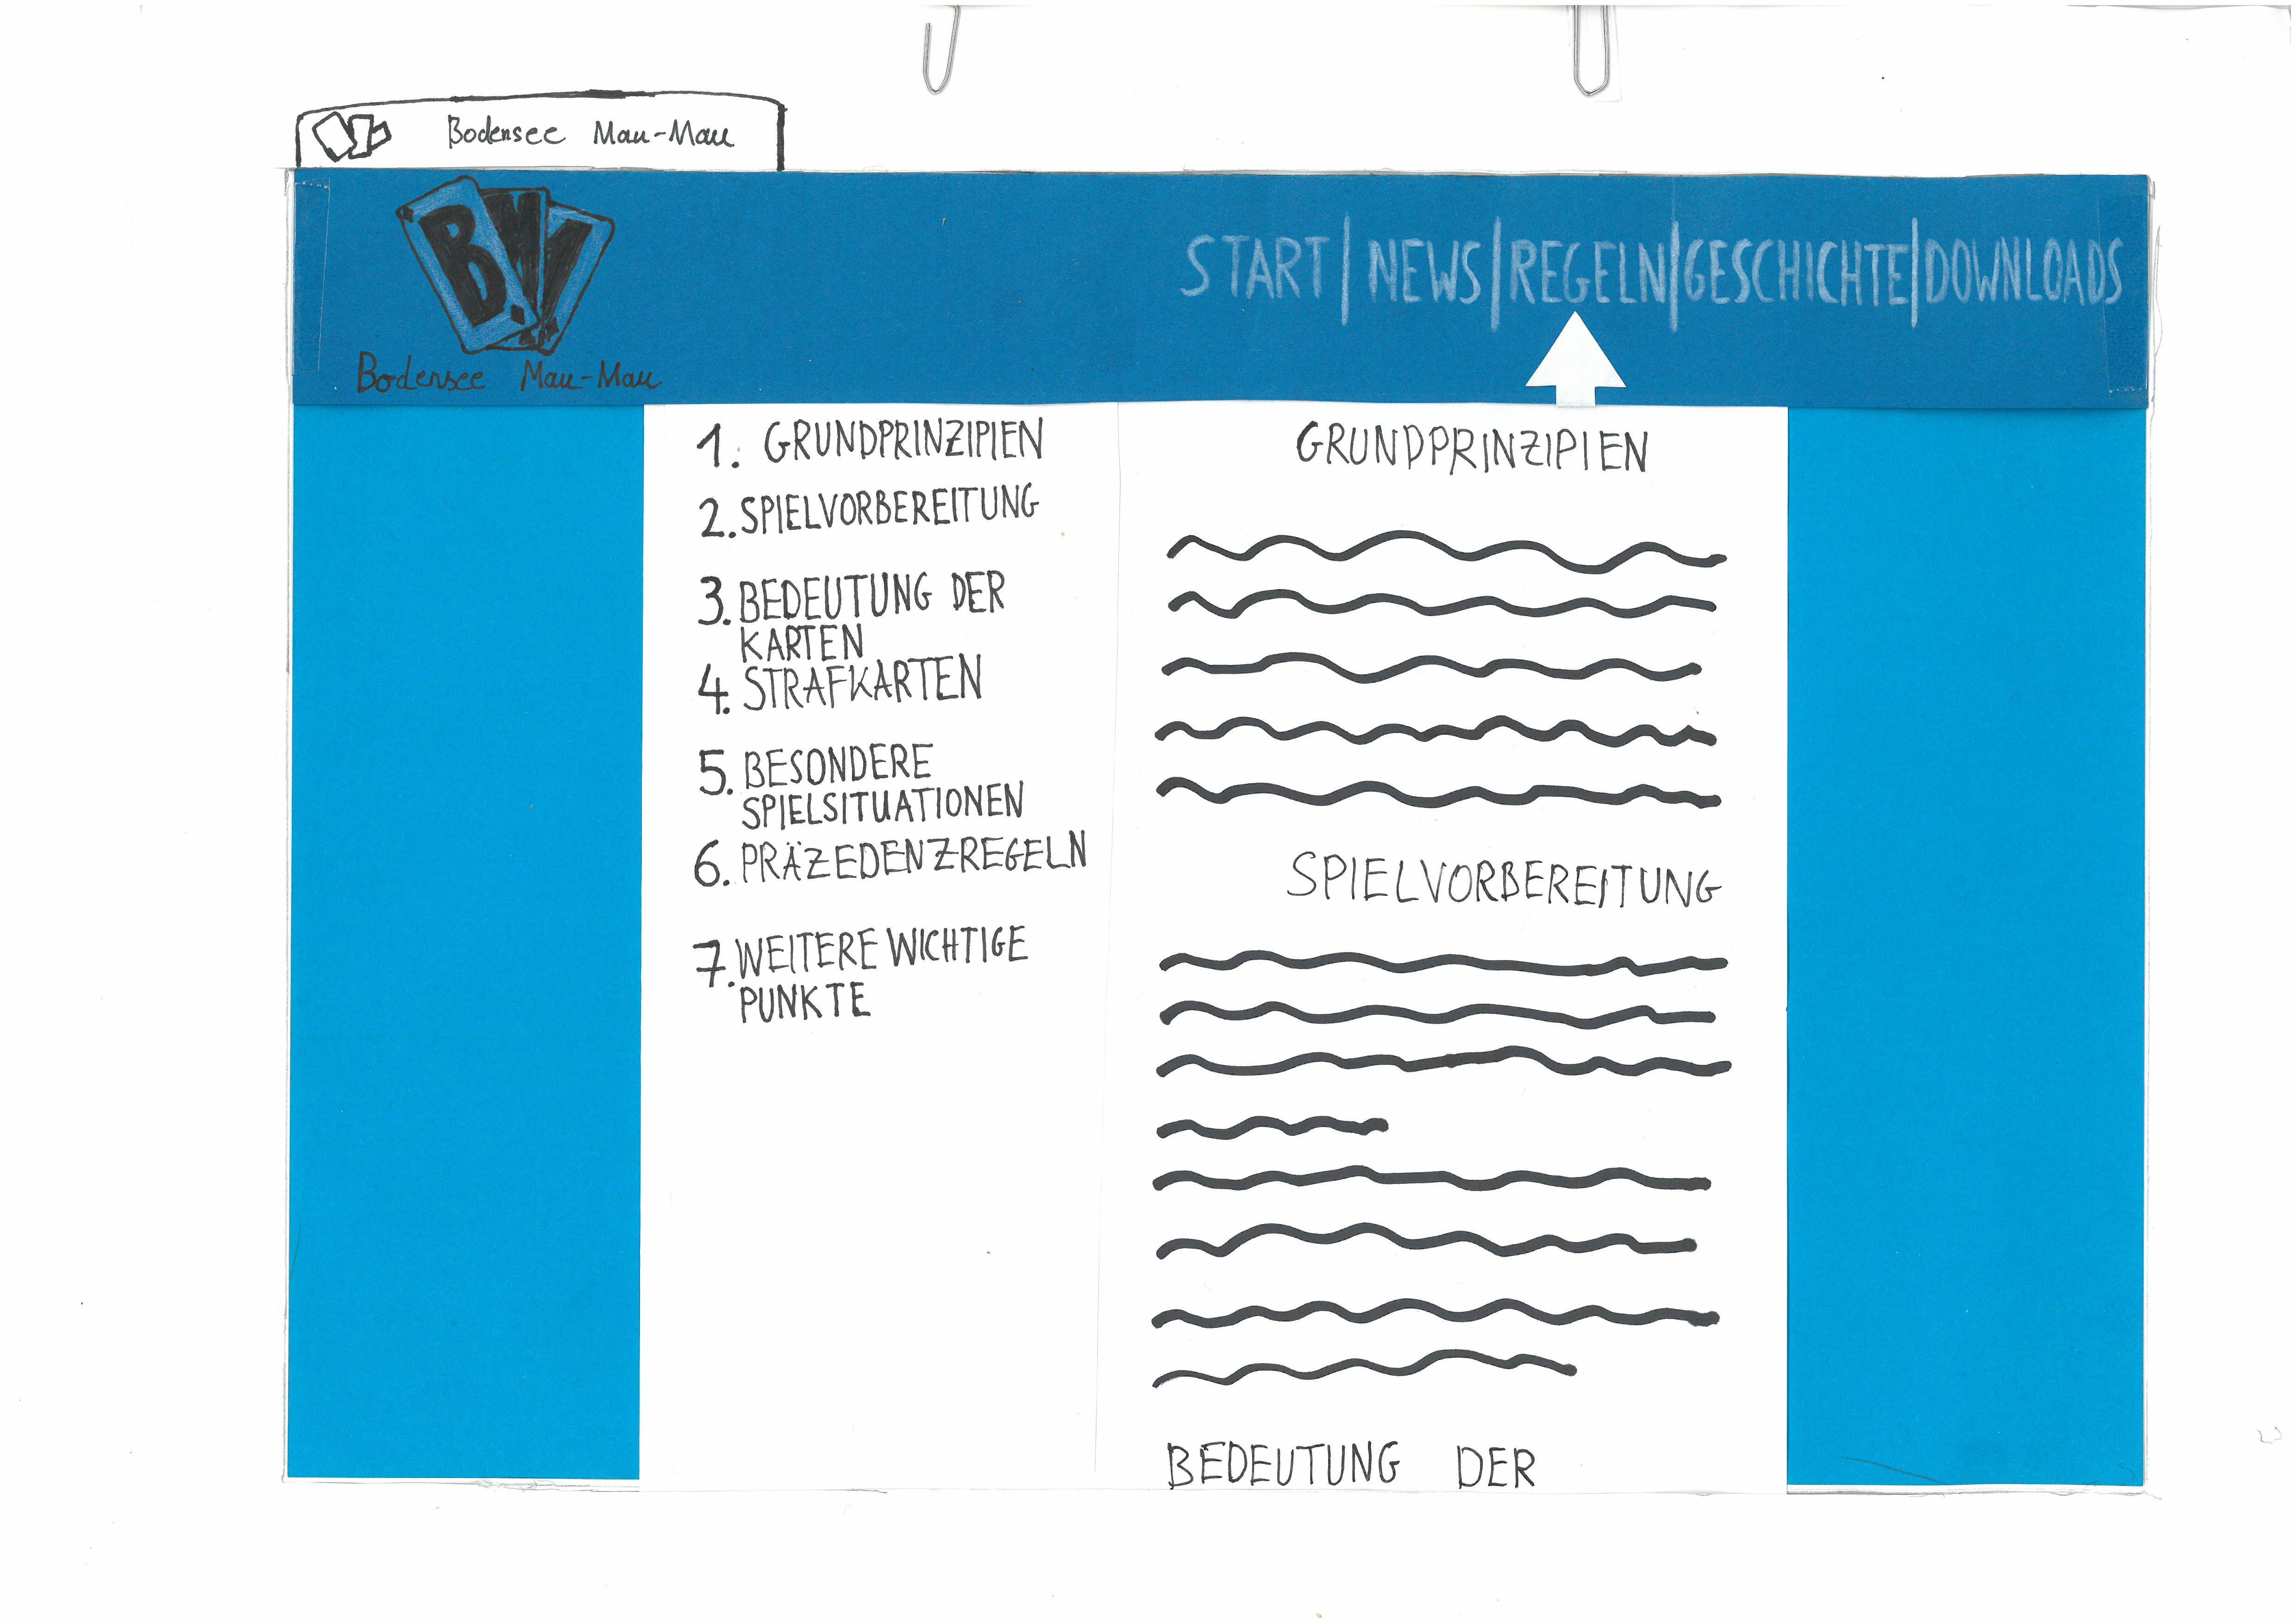
\includegraphics[width=0.9\textwidth]{regeln.jpg}
\caption{regeln.html}
 \end{center}
\end{figure}  
Die \textit{Regeln}-Seite benutzt im Gegensatz zu den anderen Seiten auf der linken Seite eine feste Navigation, zusätzlich zur oberen. Hier werden die Regeln ausführlich beschrieben und durch die zusätzliche Navigation gelangt man leicht zu einer bestimmten Regel. Manche Regeln bekommen noch Icons (aus Blatt 2), damit es interessanter wird.
\subsection*{4. Geschichte}
  \begin{figure}[H]
 \begin{center}
 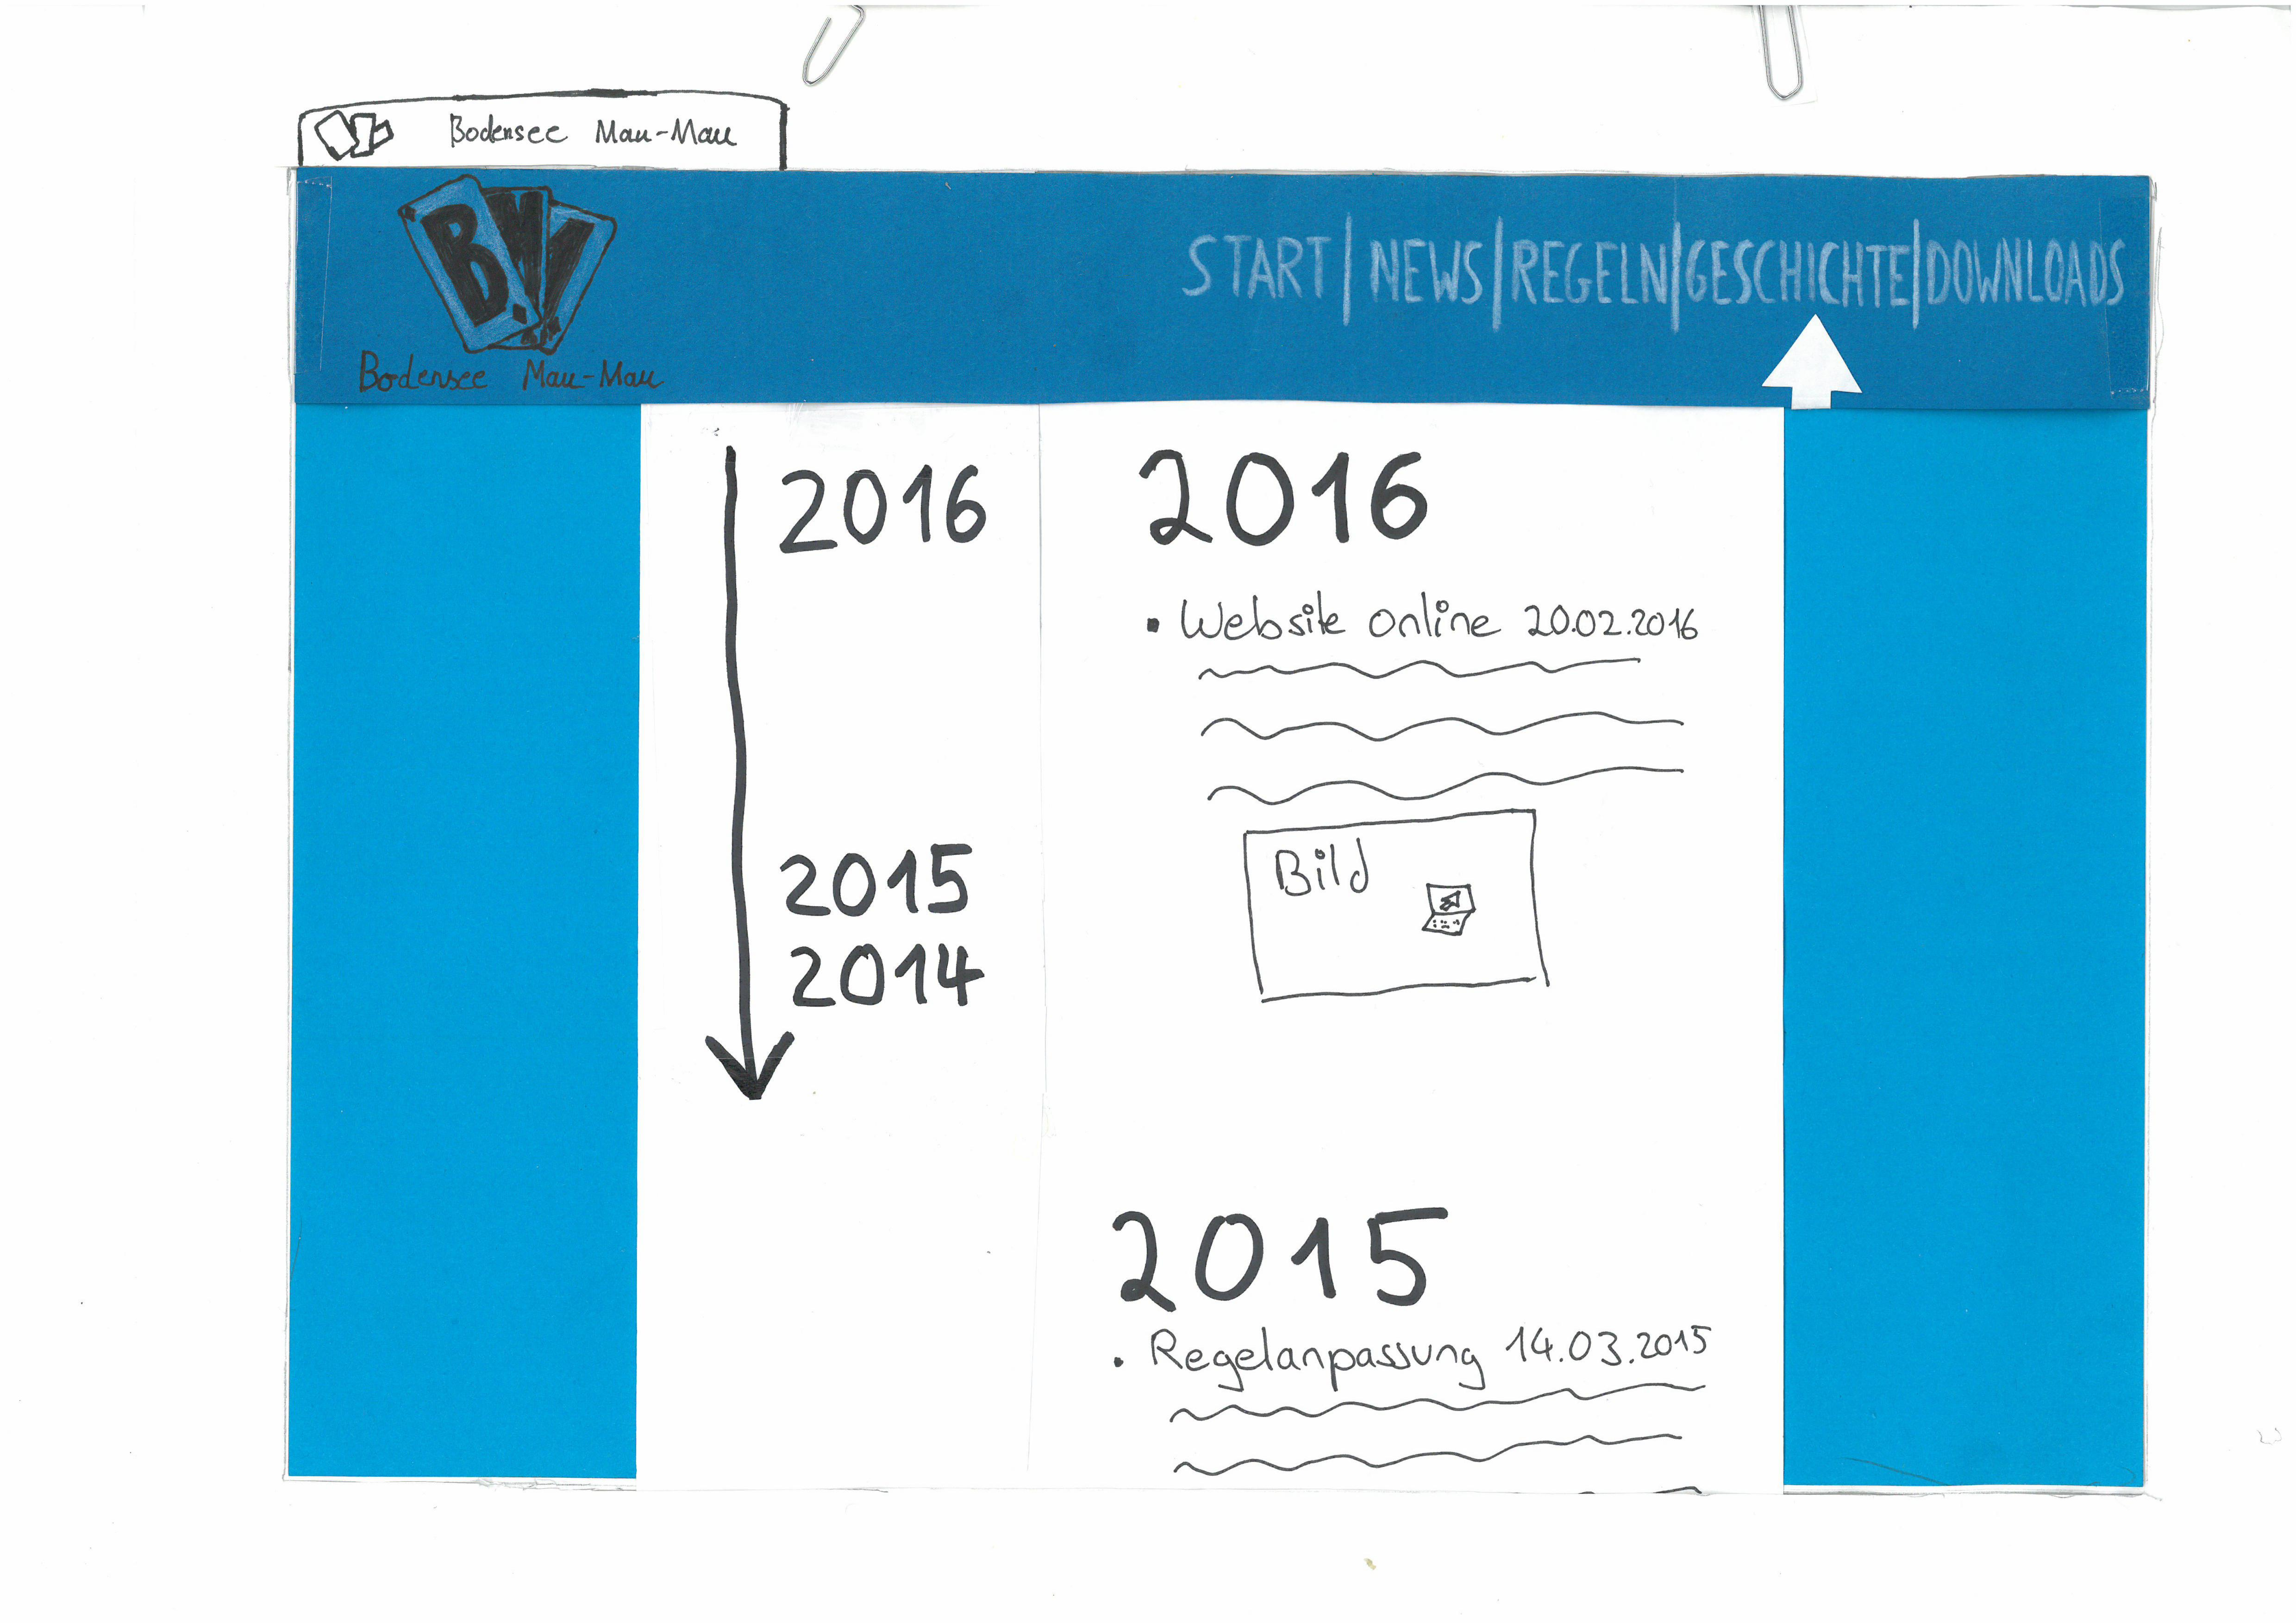
\includegraphics[width=0.9\textwidth]{geschichte.jpg}
\caption{geschichte.html}
 \end{center}
\end{figure}  
 Die \textit{Geschichte}-Seite ist zwei-geteilt. Auf der linken Seite befindet sich ein Pfeil, auf die bisherigen Jahre stehen. Die Jahre sind anklickbar, man springt dann zu dem jeweiligen Jahr.  Die linke Seite ändert sich beim Scrollen nicht. Auf der rechten Seite sind die einzelnen Einträge. Zu jedem Eintrag mit Datum folgt dann eine längere Beschreibung, was sich dort ereignet hat. Gestartet (oberster Eintrag) wird mit dem neustem geschichtlichen Ereignis (z. B. Homepage geht online), worauf dann ältere Ereignisse folgen (z. B. Spiel wurde erfunden). Die Einträge werden noch von Bildern ergänzt.

\subsection*{5. Downloads}
  \begin{figure}[H]
 \begin{center}
 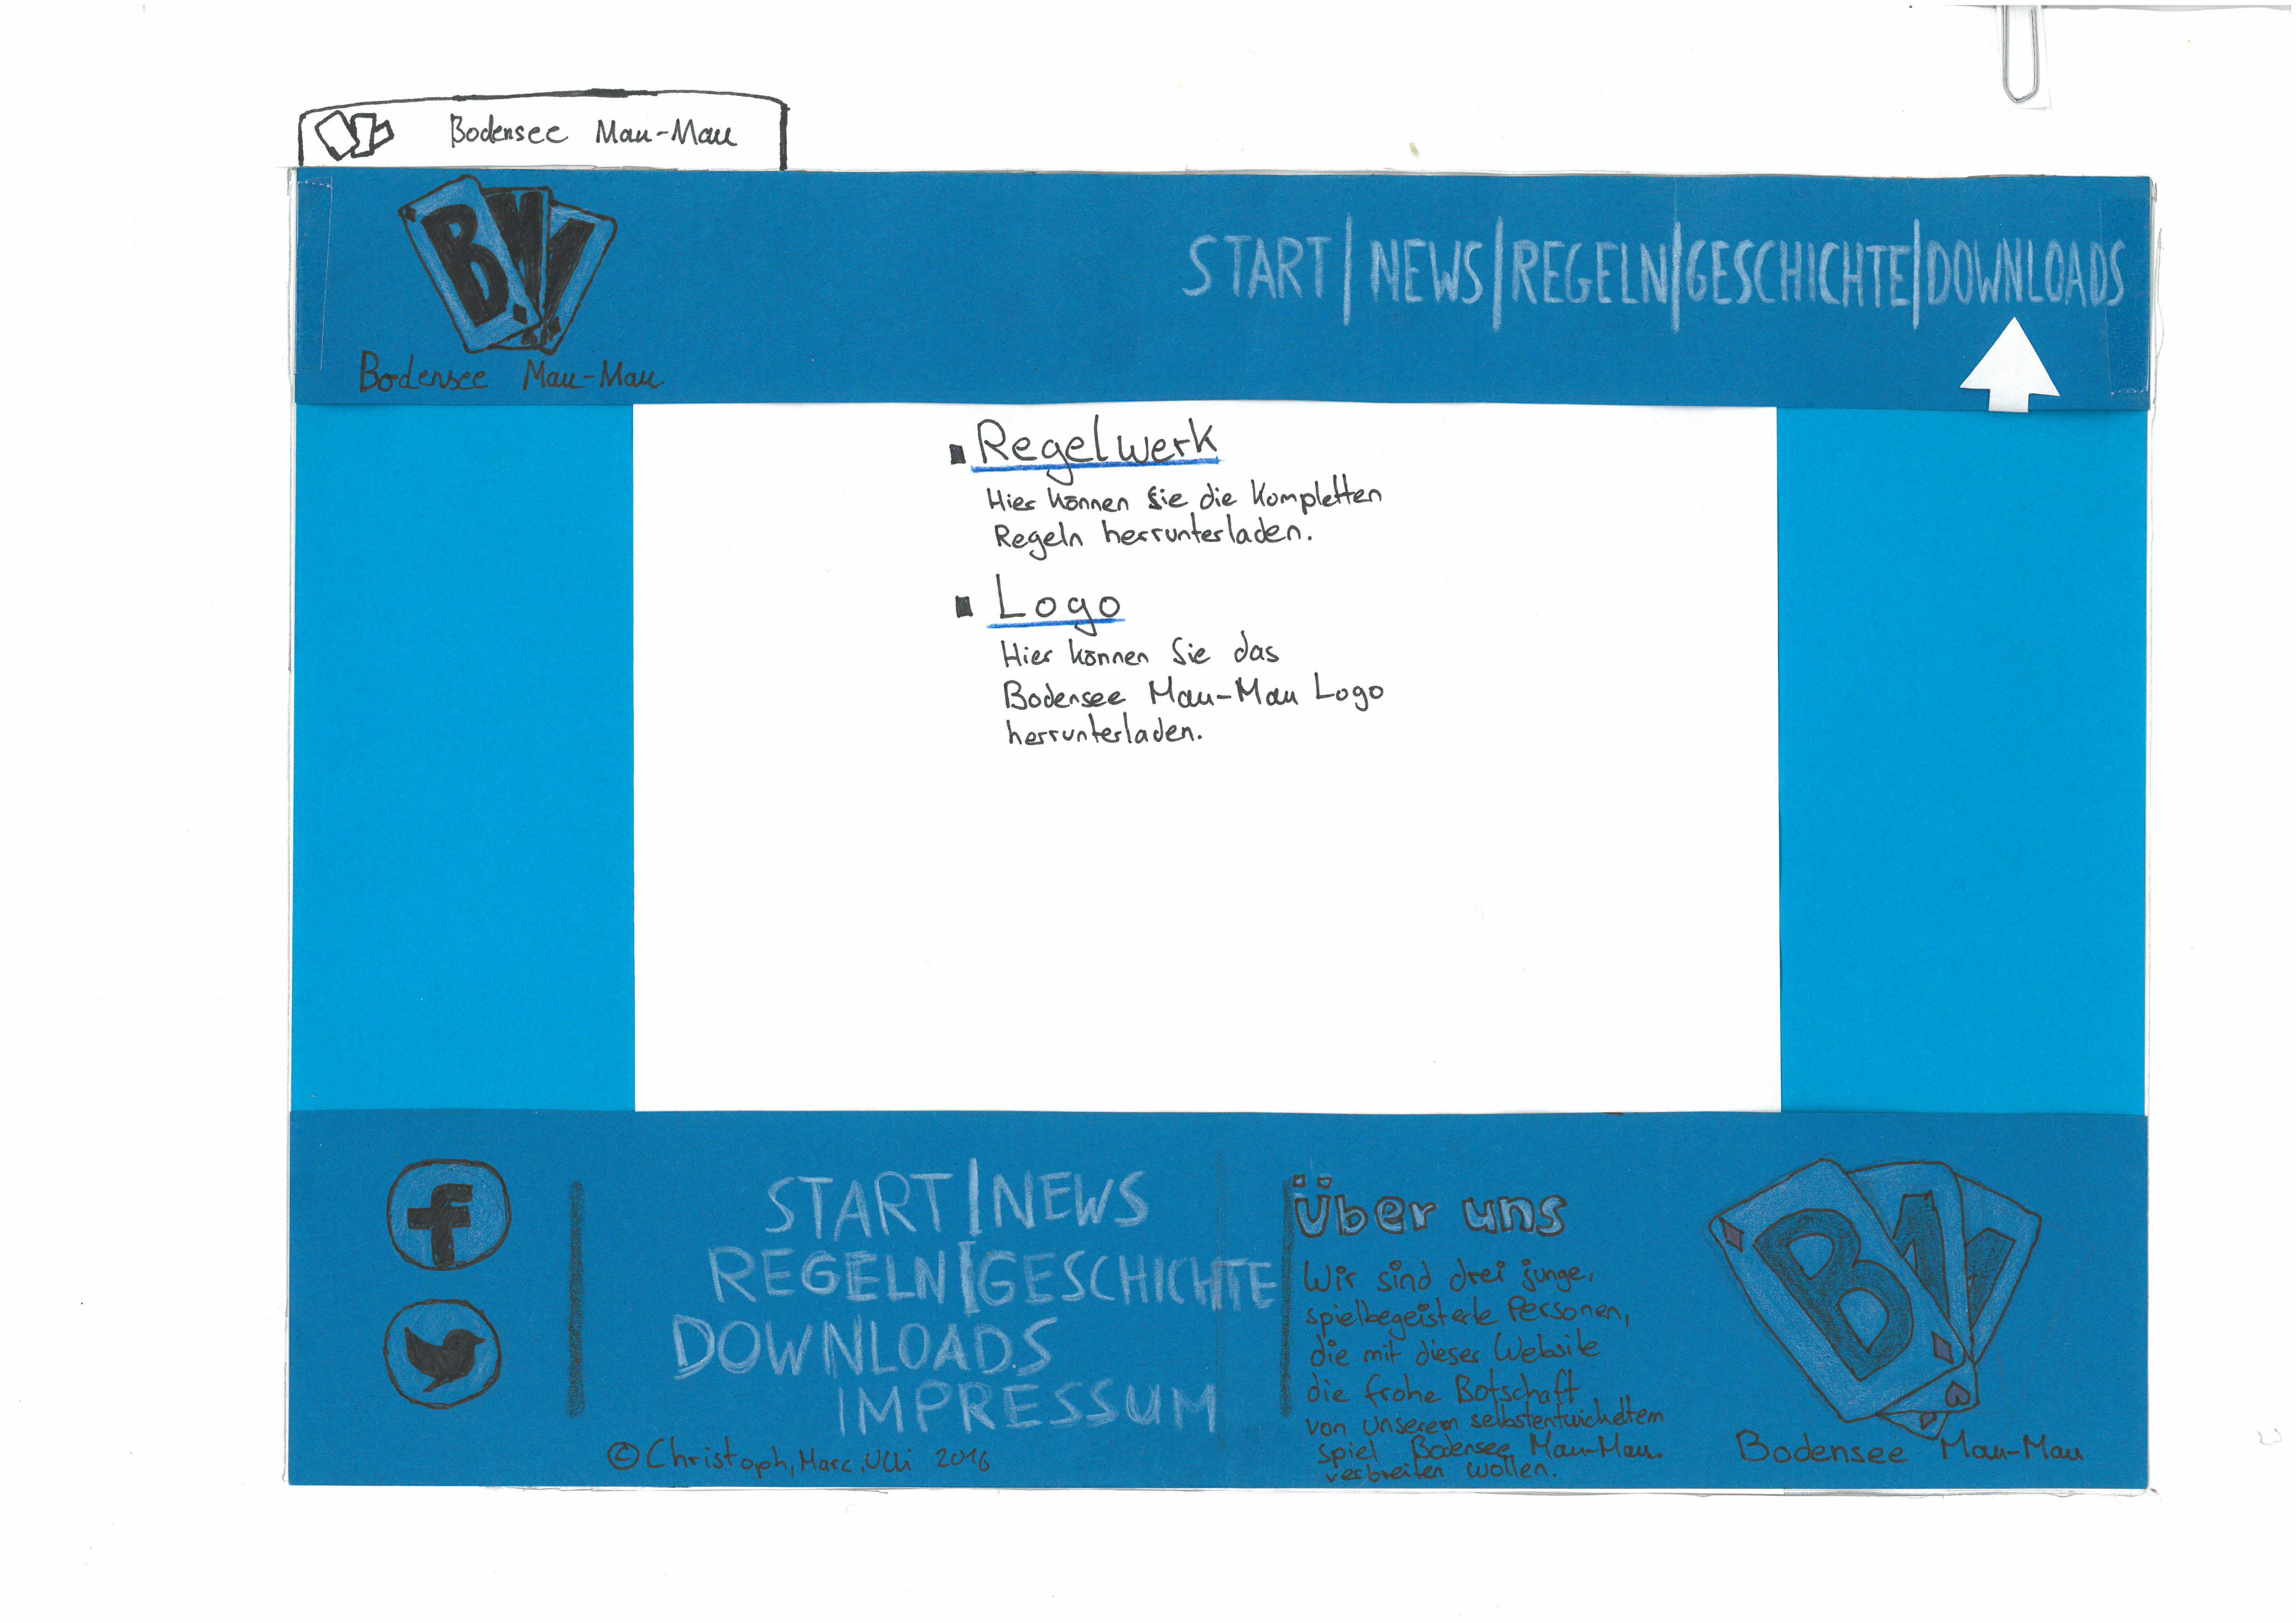
\includegraphics[width=0.9\textwidth]{downloads.jpg}
\caption{downloads.html}
 \end{center}
\end{figure}  
  Der \textit{Downloads}-Bereich soll eine einfache Auflistung des downloadbaren Dinge sein, mit je einer kurzen Beschreibung (z. B. das Regelwerk).
\subsection*{6. Impressum}
  \begin{figure}[H]
 \begin{center}
 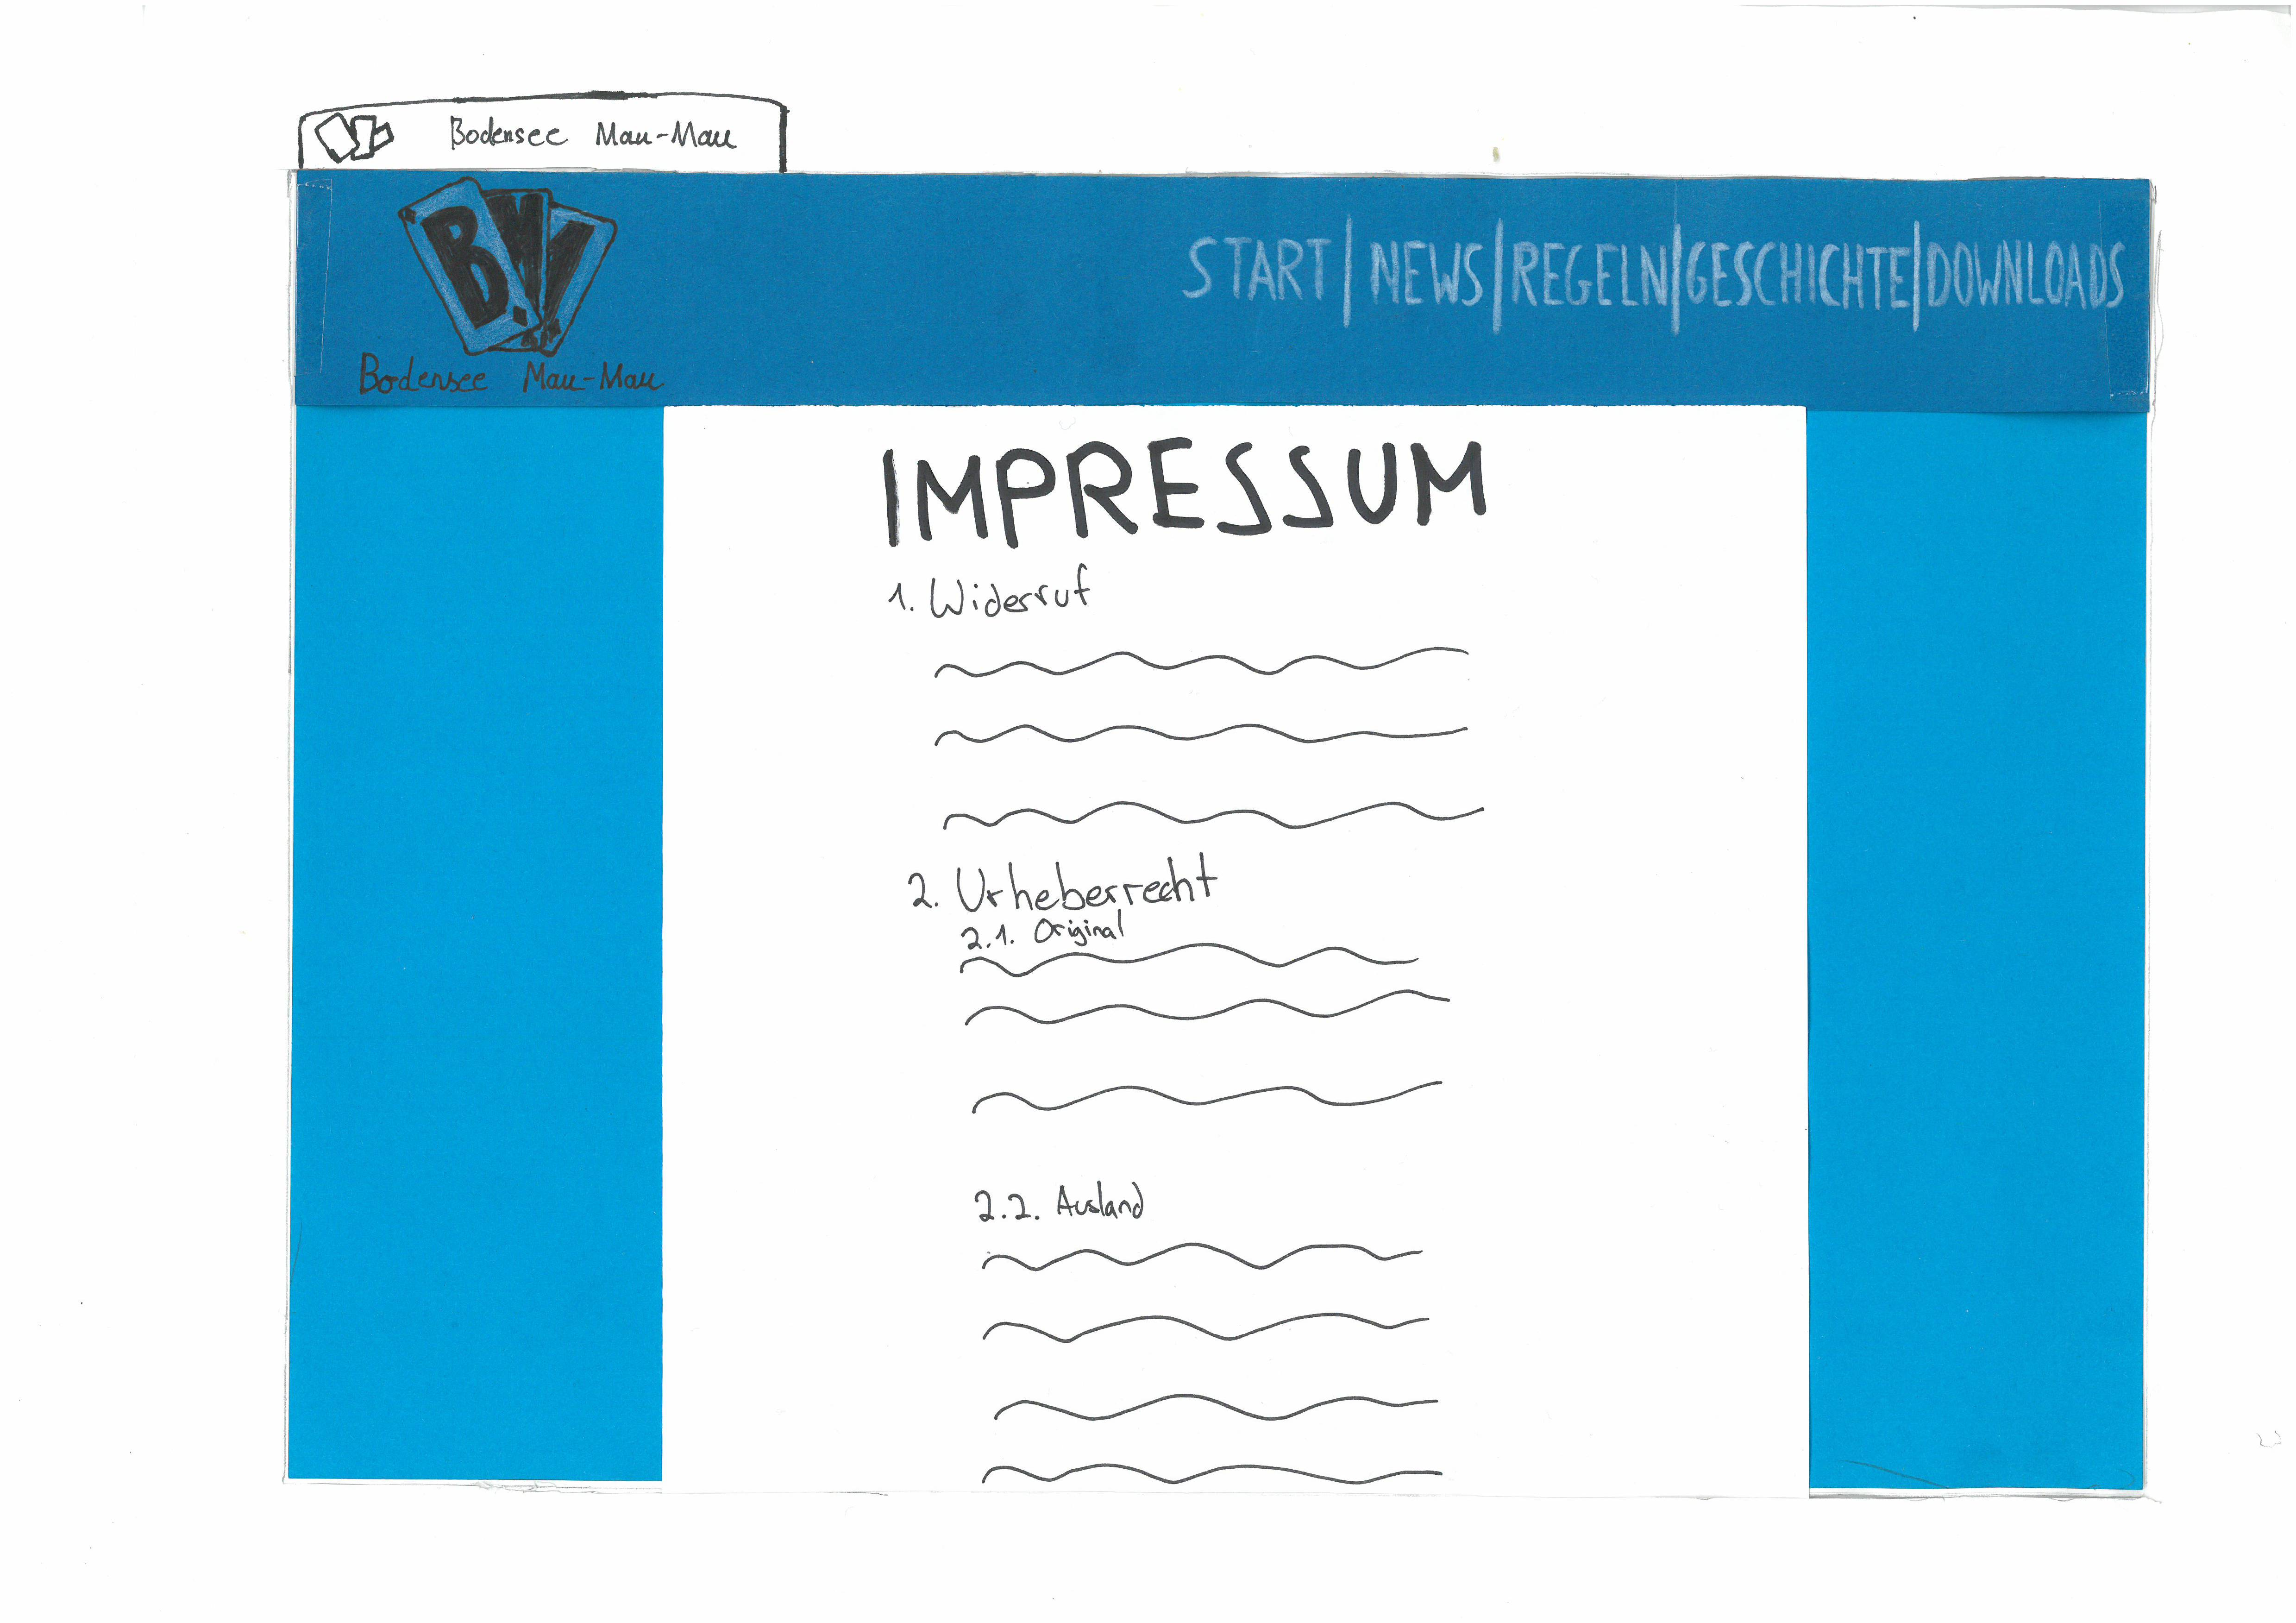
\includegraphics[width=0.9\textwidth]{impressum.jpg}
\caption{impressum.html}
 \end{center}
\end{figure}  
  Das \textit{Impressum} ist nur ein einfacher, linksbündiger Standarttext. Im Gegensatz zu den anderen Seiten hat er noch eine Überschrift: Impressum, damit sich der Nutzer besser zurecht findet.
\subsection*{Test der 3 Szenarien}
\begin{enumerate} 
\item Die Person aus Szenario 1 ist zum ersten Mal auf der Website und möchte einen Überblick bekommen. Sie sucht ein neues Unterhaltungsspiel. Auf der \textit{Startseite} steht weiter unten eine recht kurze Info über das Spiel und dessen Entstehung. Sie bekommt einen Überblick und das Interesse die Regeln zu lesen, z. B. über dem Call-To-Action über dem Infotext oder über die Navigation.
  \begin{figure}[H]
 \begin{center}
 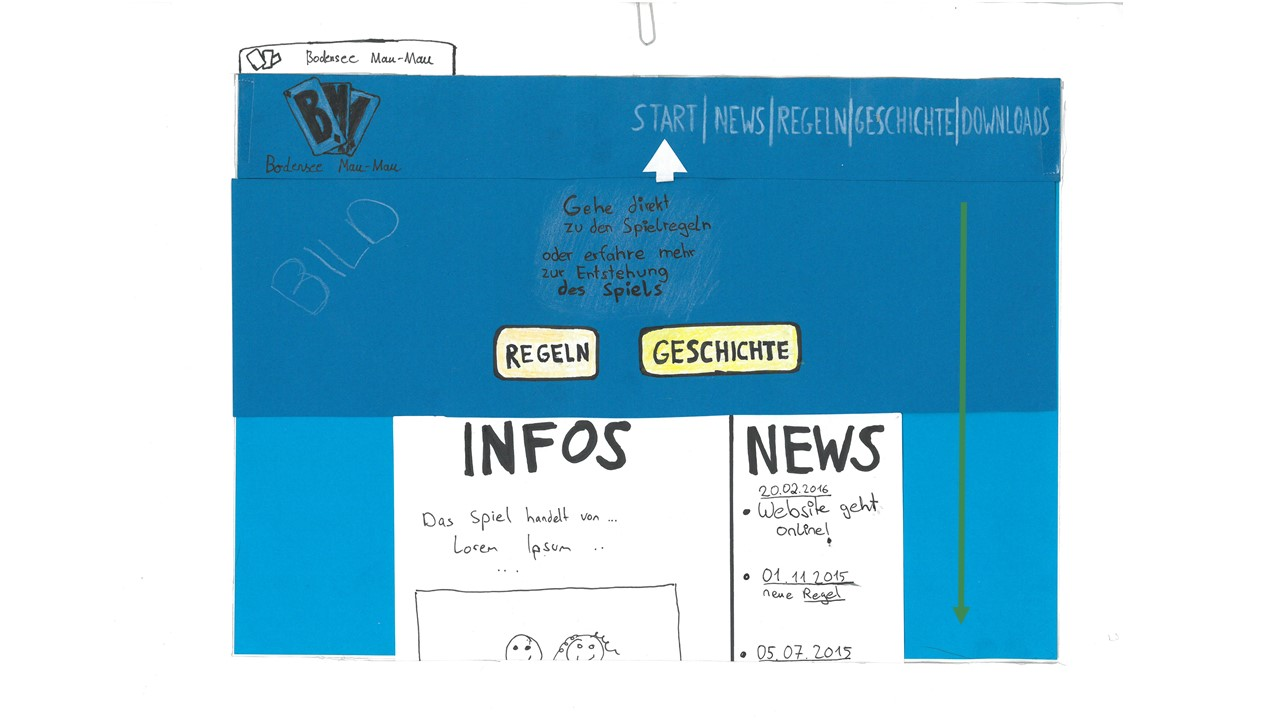
\includegraphics[width=0.7\textwidth]{szenario1-1.jpg}
\caption{\textbf{Szenario 1:} Zuerst scrollt die Person auf der Startseite runter.}
 \end{center}
\end{figure}  
  \begin{figure}[H]
 \begin{center}
 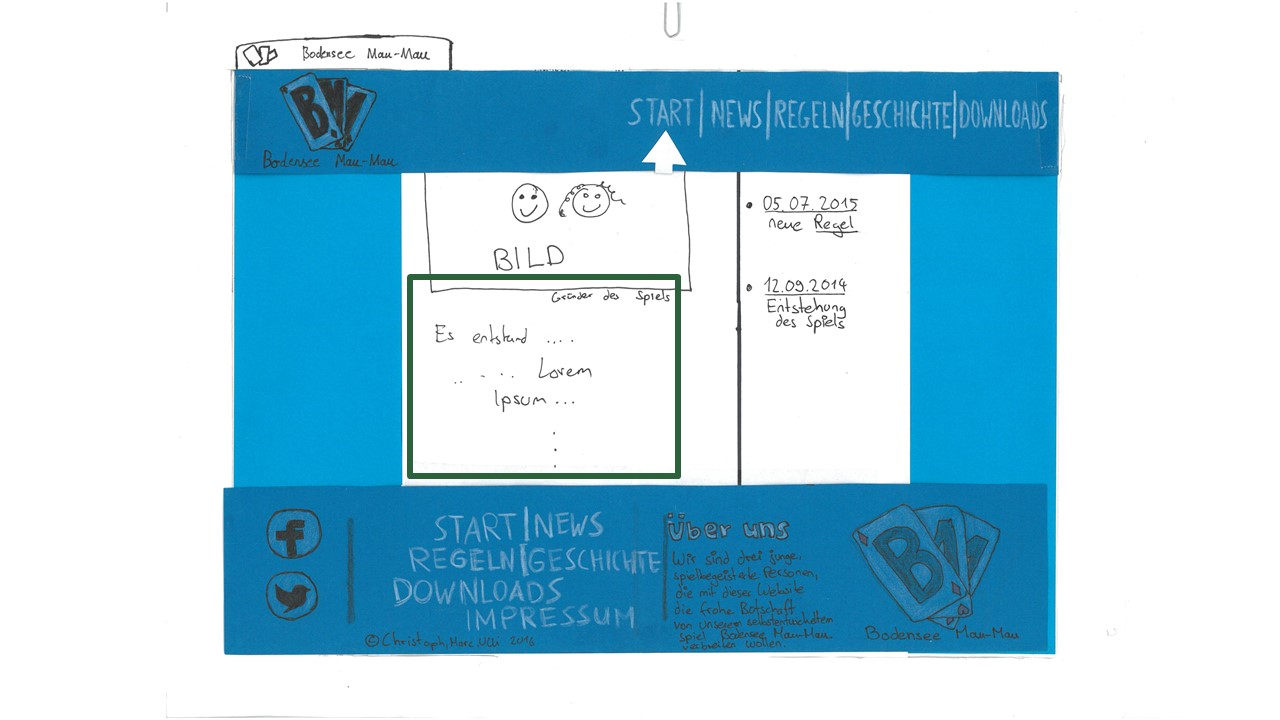
\includegraphics[width=0.7\textwidth]{szenario1-2.jpg}
\caption{\textbf{Szenario 1:} Dann liest sie den kleinen Infotext.}
 \end{center}
\end{figure}  
  \begin{figure}[H]
 \begin{center}
 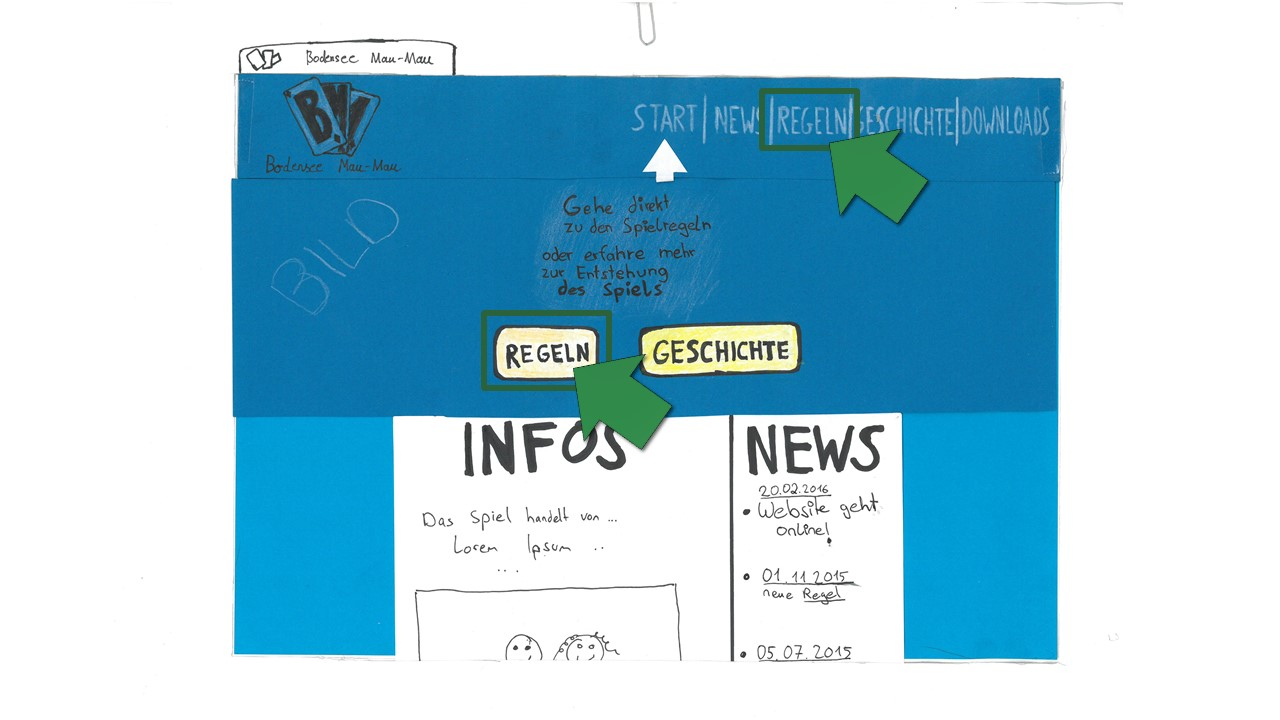
\includegraphics[width=0.7\textwidth]{szenario1-3.jpg}
\caption{\textbf{Szenario 1:} Nun möchte sie auf die \textit{Regeln}-Seite gelangen.}
 \end{center}
\end{figure}  
\item Die Person aus Szenario 2 möchte zu den \textit{Regeln} gelangen, um eine bestimmte Regel nachzuschauen. Sie kennt das Spiel, kann sich jedoch nicht mehr an alle Regeln erinnern. Sie kommt über den Call-To-Action zu ihrem Ziel, sowie über die obere Navigationsleiste. Bei \textit{Regeln} kann sie dann über die linke Navigationsleiste direkt zu der gewünschten Regel springen und ist zufrieden.
\begin{figure}[H]
 \begin{center}
 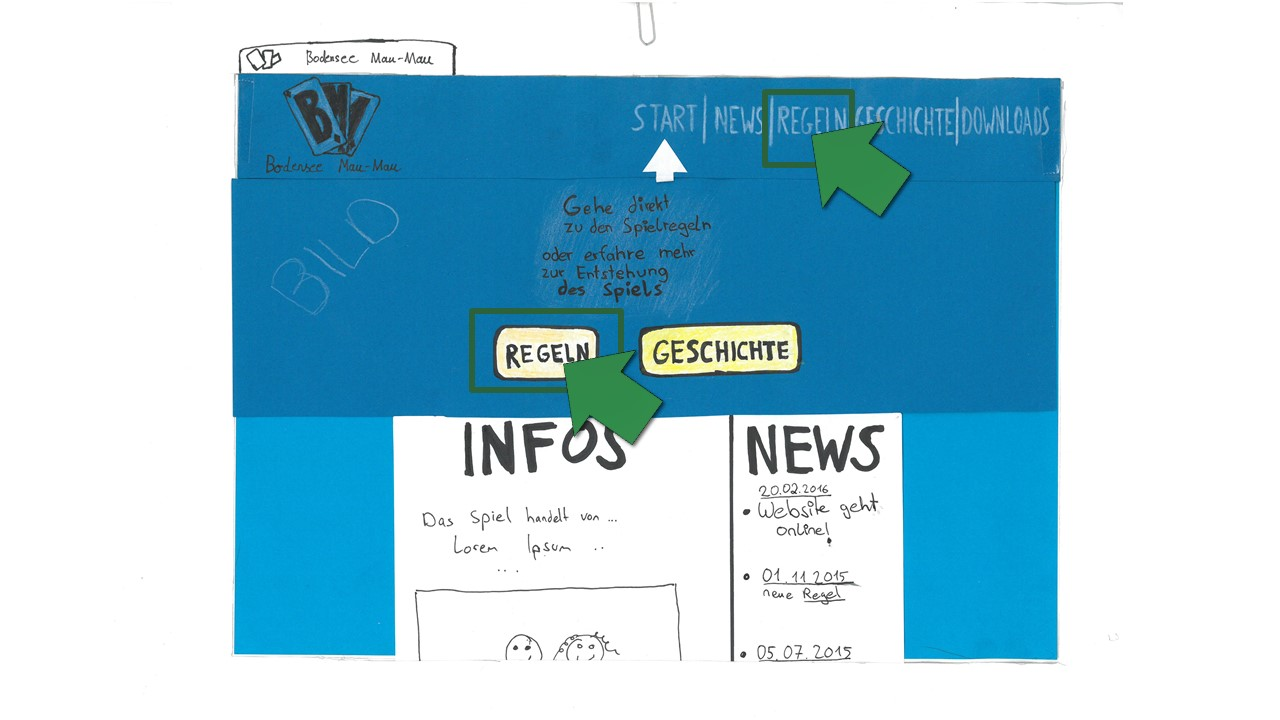
\includegraphics[width=0.7\textwidth]{szenario2-1.jpg}
\caption{\textbf{Szenario 2:} Zuerst möchte die Person auf \textit{Regeln} gelangen.}
 \end{center}
\end{figure}  
\begin{figure}[H]
 \begin{center}
 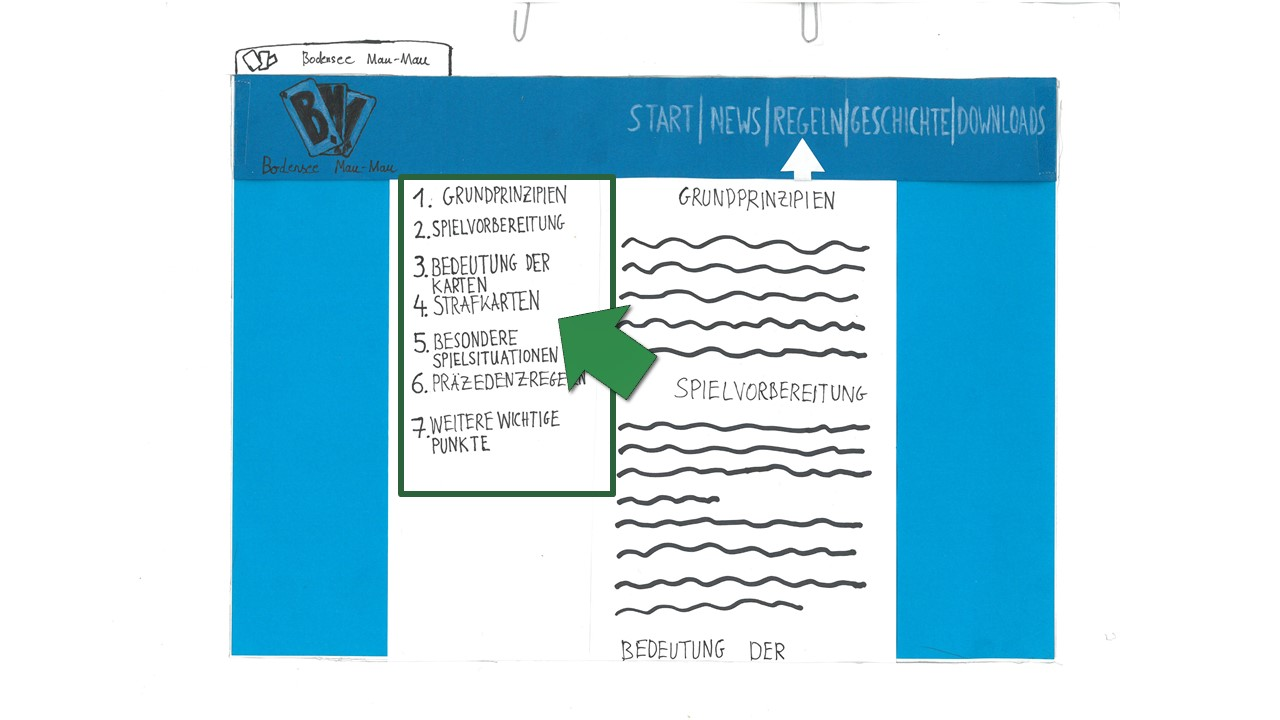
\includegraphics[width=0.7\textwidth]{szenario2-2.jpg}
\caption{\textbf{Szenario 2:} Bei \textit{Regeln} möchte sie nun eine bestimmte Regel finden.}
 \end{center}
\end{figure}  
\item Die Person aus Szenario 3 möchte die aktuellsten Neuigkeiten erfahren. Sie kennt das Spiel und besucht öfters die Website. Diese werden schon auf der \textit{Startseite} rechts in einer Infobox eingeblendet. Möchte sie diese ausführlicher lesen, so kann sie über diese Box (z. B. auf die einzelnen Einträge klicken, oder auf die Überschrift \textit{News}), oder über die obere Navigationsleiste zu \textit{News} gelangen. Dort sieht sie sofort oben die neusten News und kann so lange runterscrollen, bis sie die Einträge schon kennt.
\begin{figure}[H]
 \begin{center}
 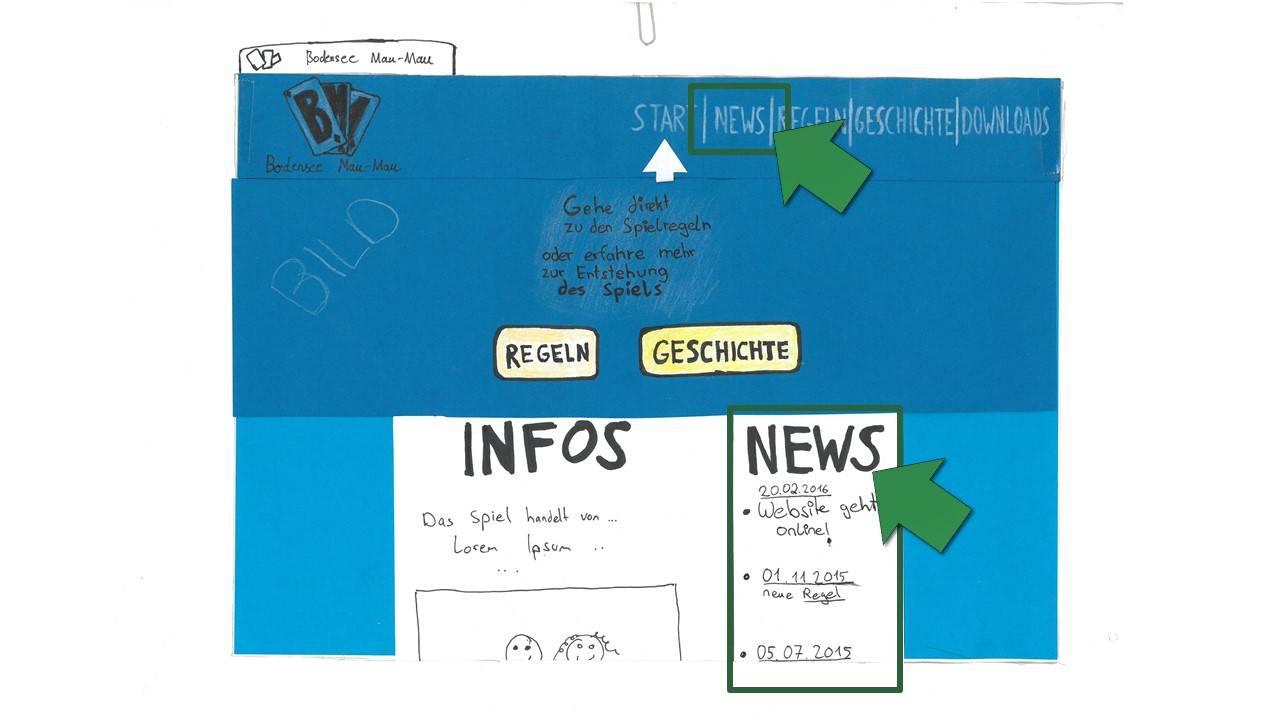
\includegraphics[width=0.7\textwidth]{szenario3-1.jpg}
\caption{\textbf{Szenario 3:} Auf der Startseite sieht die Person Überschriften der neusten Neuigkeiten und möchte dann auf die Seite \textit{News}.}
 \end{center}
\end{figure}  
\begin{figure}[H]
 \begin{center}
 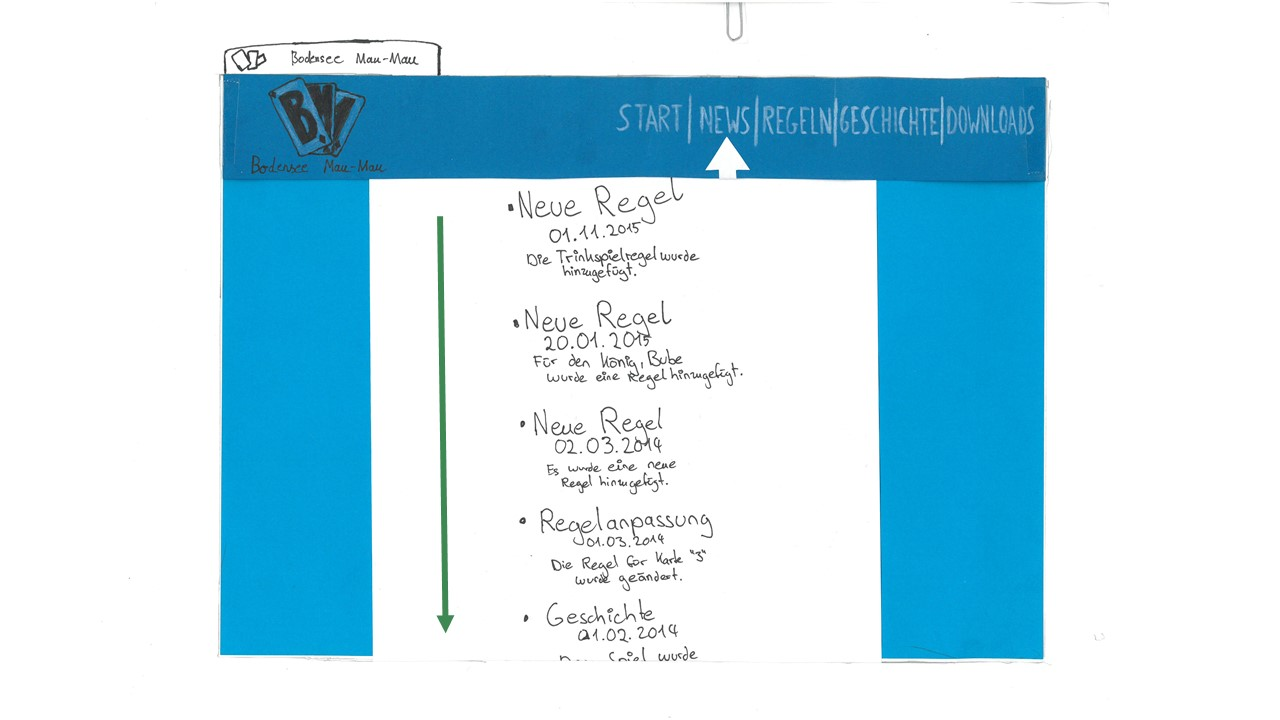
\includegraphics[width=0.7\textwidth]{szenario3-2.jpg}
\caption{\textbf{Szenario 3:} Dort scrollt sie bis sie die Einträge kennt runter.}
 \end{center}
\end{figure}  
\end{enumerate}
Der Papierprototyp hat alle 3 Szenarien bestehen können. 
\section*{Aufgabe 6: Heuristische Evaluation}
\subsection*{a) Durchführung der heuristischen Evaluation}
\begin{enumerate}
\item Gewählte Heuristiken:
\begin{description}
\item[Heuristik 1:] Übereinstimmung zwischen dem System und der realen Welt
\item[Heuristik 2:] Konsistenz und Standards
\item[Heuristik 3:] Sichtbarkeit des Systemstatus
\item[Heuristik 4:] Benutzerkontrolle und Freiheit
\item[Heuristik 5:] Wiedererkennen, statt sich erinnern
\end{description}

\item Durchführungen der Heuristiken:
\begin{description}
\item[Heuristik 1 (Übereinstimmung zwischen dem System und der realen Welt):] \ \\ Der nicht deutschsprachige Tester der Heuristik ruft die Seite über seinen Browser auf.
Ihm fällt anhand des geschrieben Textes sofort auf, dass es sich um eine deutschsprachige Seite handelt. Er schaut sich um, ob es möglich ist irgendwo die Sprache zu ändern. Er wird nicht fündig, klickt über die Navigation auf \textit{Geschichte} und findet noch mehr deutschen Text vor und wieder keine Möglichkeit die Sprache zu ändern. Er verwendet nun das Übersetzungsprogramm des Browsers, was aber nicht besonders gut übersetzt. Bald darauf bricht er ohne wirklichen Informationsgewinn den Besuch der Seite ab.
\item[Heuristik 2 (Konsistenz und Standards):]\ \\
Der Tester der Heuristik ruft die Seite über seinen Browser auf. Er sucht die Seite nach uneindeutigen Informationen ab und erkennt, dass Regeln und Geschichte sowohl in der Header
Leiste als auch auf den beiden Buttons auf dem Call-to-Action stehen. Beim runter Scrollen stellt er fest, dass der Header
fixiert ist und als er am Footer ankommt, dort die selben Informationen wie in der Navigation vorzufinden sind. Es wurden also Uneindeutigkeiten an zwei Stellen ausfindig gemacht.
\item[Heuristik 3 (Sichtbarkeit des Systemstatus):] \ \\
Der Tester der Heuristik ruft die Seite über seinen Browser auf. Er landet zunächst auf der \textit{Start}-Seite, verweilt eine Weile auf der Seite und scrolled auch nach unten. Nachdem er überzeugt ist alles gesehen zu haben, wechselt er über den Button "Regeln"\ auf die \textit{Regeln}-Seite. Hier erkennt er, dass die Verlinkung „Regeln“ im Header hervorgehoben wurde. Er sucht nach der Regel für die Spielkarte „5“ und wechselt danach über die Verlinkung in der Navigation auf die \textit{Geschichte}-Seite. Nun fällt ihm auf, dass die Verlinkung „Geschichte“ in Header hervorgehoben wurde und die Hervorhebung von „Regeln“ wieder verschwunden ist. Der Tester schließt daraus, dass die Hervorhebung Auskunft über den aktuellen Systemstatus gibt. 
Bei der \textit{Impressum}-Seite findet keine Hervorhebung in der Navigation statt, dafür erscheint eine Überschrift auf der aufgerufenen Seite, so dass der Tester weiß, wo er sich gerade befindet.
Die Anforderungen der Heuristik können also als erfüllt angesehen werden.
\item[Heuristik 4 (Benutzerkontrolle und Freiheit):] \ \\
Der Tester der Heuristik ruft die Seite über seinen Browser auf. Er landet zunächst auf der Startseite, verweilt eine Weile auf der Seite und scrollt auch nach unten. Nachdem er überzeugt ist
alles gesehen zu haben, wechselt er über den Regeln-Button auf die \textit{Regeln}-Seite. Nachdem er die Regel für die Spielkarte „10“ nachgeschaut hat, wechselt auf die Seite \textit{Geschichte}. Auf der Seite \textit{Geschichte} liest er die Entstehungsgeschichte des Spiels nach. Mit einem Mal fällt ihm ein, dass er auch die Regel der Spielkarte „3“ nochmals nachschauen möchte. Er geht also über „Regeln“ in der Navigation nochmals auf die Seite \textit{Regeln} zurück und schaut die Regel nach. Anschließend wechselt er analog auf die Startseite und danach auf die \textit{Impressum}-Seite, bevor er seinen Besuch der Seite beendet.
Die Anforderungen der Heuristik können also als erfüllt angesehen werden, denn der Nutzer kann zu jeder Zeit auf jede Seite über die Verlinkung in der fixierten Navigation, bzw. über die Verlinkungen im Footer wechseln.
\item[Heuristik 5 (Wiedererkennen, statt sich erinnern):] \ \\ Der Tester der Heuristik ruft die Seite über seinen Browser auf. Er landet zunächst auf der Startseite, verweilt eine Weile auf der Seite und scrolled auch nach unten. Nachdem er überzeugt ist
alles gesehen zu haben, wechselt er auf die Seite „Regeln“. Danach gelangt er, aufgrund der Unternavigation auf linken Seite, schnell zur gesuchten Regel „Ruf-Hierarchie“. Danach wechselt auf die Seite \textit{News}. Hier sucht er wann die Regel „Ruf-Hierarchie“ eingeführt wurde. Er stellt fest, dass die Regel auf jeden Fall nicht erst kürzlich eingeführt wurde (da auf der \textit{News}-Seite die neusten Regeln oben stehen). Der Tester scrollt mehr oder weniger per Zufall etwas nach unten und dann wieder nach oben und sucht mehr oder weniger per Zufall ob er irgendwo über die gesuchte Regel stolpert. Irgendwann scrolled er ganz nach unten und entdeckt, dass die Regel zu den Gründungsregeln gehört. Die Heuristik wurde erfüllt.
\end{description}
\textbf{Gefundene Probleme:}
\begin{itemize}
\item Uneindeutigkeit von den Buttons des Call-to-Action und der Navigation und dem Footer
\item Kein Feedback beim Download
\item Fremdsprachige Besucher können die Seite nicht nutzen
\end{itemize}

\item Bewertungen der Heuristiken:\\ 
Zur Bewertung wie schwerwiegend ein Problem ist, wurde eine Skala von 0 – 10 verwendet. Im
Grad aufsteigend ist 0 das am wenigsten schwerwiegend und 10 am schwerwiegendsten.
\begin{description}
\item[Heuristik 2 (Konsistenz und Standards):] \ \\
Das Problem der Unklarheit über die Eindeutigkeit ist das bisher schwerwiegendste Problem.
Der Nutzer könnte sich evtl. unsicher sein, ob der Link zu \textit{Regeln} und \textit{Geschichte} am oberen Bildschirmrand zu den gleichen Seiten führt, wie die beiden Buttons, auf denen ebenfalls jeweils Regeln bzw. Geschichte steht.
Genau so befinden sich dieselben Verlinkung zu allen Seiten sowohl in der Navigation, als auch im Footer, was bei einer fixierten Navigation dazu führt, dass sich beide Verlinkungen im Sichtfeld des Besuchers befinden, wenn bis zum Footer runter gescrollt wurde.\\
Bewertung : 7
\item[Heuristik 1 (Übereinstimmung zwischen dem System und der realen Welt):] \ \\
Weitestgehend ist diese Heuristik erfüllt. Die Seite ist vorrangig dafür konzipiert, dass ein Jugendlicher/Erwachsener sie über PC/Laptop usw. aufruft und mit ihr interagiert. Ein einziger Konflikt mit der
realen Welt ist, dass der Nutzer evtl. nicht deutschsprachig ist und die Seite nur auf deutsch einsehbar ist.\\
Bewertung: 4
\item[Heuristik 5 (Wiedererkennen, statt sich erinnern):] \ \\
Die Heusitik wurde weitgehend erfüllt, ein kleines Problem könnte beim Download einer Datei auftreten, dass sich z. B. der Nutzer nicht mehr daran erinnern kann, was er runtergeladen hat.
Bewertung: 3
\item[Heuristik 3 (Sichtbarkeit des Systemstatus):] \ \\
Diese Heuristik ist weitgehend erfüllt. Am oberen Bildschirmrand wird markiert, auf welcher Seite sich der Besucher der Seite gerade befindet. Nur beim Impressum unterscheidet sich die Sichtbarkeit des Systemstatus von den anderen Seiten, sie ist aber dennoch durch eine Überschrift vorhanden.\\
Bewertung: 1
\item[Heuristik 4 (Benutzerkontrolle und Freiheit):] \ \\
Heuristik ist erfüllt. Der Besucher der Seite kann über die Verlinkungen im fixierten Header bzw. Footer von jeder Seite aus zu allen anderen Seiten gelangen.\\
Bewertung: 0
\end{description}

\item Verbesserungsvorschläge
\begin{description}
\item[Heuristik 1 (Übereinstimmung zwischen dem System und der realen Welt):] \ \\
Eine Einstellung der Sprache könnte noch hinzugefügt werden, zumindest wichtige Sprachen (Weltsprachen) wie Englisch, Spanisch, Russisch und Französisch. Damit der fremdsprachige Besucher der Seite sofort herausfindet wie die Sprache geändert werden kann, könnten z.B. kleine
Flaggen in der Navigation angezeigt werden, oder ein paar gefächerte kleine Flaggen angebracht werden, über welche dann ein Menü aufgeklappt wird, in dem die Sprache ausgewählt werden kann.
\item[Heuristik 2 (Konsistenz und Standards):] \ \\
Es bietet sich an, die identischen Verlinkungen in Footer und der festen Navigation nur in einem von beiden zu realisieren. Das Gleiche gilt für die Buttons auf der Startseite. Diese könnten weggelassen und die Eindeutigkeit somit vollständig hergestellt werden.
\item[Heuristik 3 (Sichtbarkeit des Systemstatus):] \ \\
Man könnte das Impressum mit in die obere Navigation mit aufnehmen.
\item[Heuristik 4 (Benutzerkontrolle und Freiheit):] \ \\
Keine Probleme gefunden.
\item[Heuristik 5 (Wiedererkennen, statt sich erinnern):] \ \\
Nach einem Download kann eine entsprechende Rückmeldung ausgegeben werden. 
\end{description}
\end{enumerate}
\subsection*{b) Dokumentation von Änderungen für erste Version der Webseite}

Durch das Feedback unserer Präsentation und der durchgeführten heuristischen Evaluation, haben sich folgende Änderungen ergeben:
\begin{itemize}
\item Die Seite \textit{News} wird nicht realisiert, da die Informationen die diese Seite bereitstellen würde, bereits auf der Startseite vorhanden sind.
\item Die Buttons (der gesamte Call-to-Action) fällt weg.
\item Die Navigation im Footer wird, bis auf das Impressum, entfernt. Der Grund dafür ist, dass das Impressum für den Durschnittsbesucher nicht besonders interessant ist, doch aus rechtlichen Gründen auf jeden Fall vorhanden sein muss.
\item Der beschreibende Satz "Über uns"\ wird ebenfalls aus dem Footer entfernt und bekommt einen eigenen Abschnitt auf der Startseite.
\item Nach jedem Download erscheint eine Rückmeldung in Form eines Satzes, wie z. B. "Der Download der Datei [\textit{xy}] war erfolgreich.".
\item Damit es eine Möglichkeit zur Interaktion zwischen Besuchern und der Webseite gibt, wird noch eine \textit{Fan}-Seite hinzugefügt. Auf dieser können Vorschläge und Ideen für eigene Spielvarianten über ein Formular eingereicht werden und Bilder vom Spielen (die zuvor per E-Mail geschickt wurden) angeschaut werden.
\item Für nicht-digitale Werbung wird es noch die Möglichkeit geben, einen Flyer herunterzuladen.
\item Die Möglichkeit die Sprache zu ändern, kommt wegen des zu hohen Aufwands noch nicht mit rein. Wir merken es uns aber für den Ausblick in \textbf{Aufgabe 10}.
\end{itemize}

\section*{Aufgabe 7: Umsetzung des Projekts}
\subsection*{b) Erste Version der Webseite}
\begin{enumerate}
\item Entwicklung der Website

Neues Zeug (was während dem coden dazu kam): Sprung zum Seitenanfang, Vorschau bei Downloads, anderes Logo als im Papierprototypen

Bilderanleitung
\item Überprüfung der Funktionalitäten + Szenarios
Funktionalitäten: alle Links wurden Überprüft, sowie der Code geordnet und mit IntelliJ IDEA 2016.2.4 überprüft. 
%\begin{figure}[H]
% \centering
%   \includegraphics[width=0.7\textwidth]{Szenario1.png}
%\caption{Szenario 1, Schritt 1}
%\end{figure}

\end{enumerate}
\section*{Aufgabe 8: Prüfung der Barrierefreiheit}
Für den Test auf Barrierefreiheit wurde \textbf{WebsiteV1} verwendet.
Das Ergebnis des Barrierefreiheit Tests fiel mit 90,5 von 100 erreichbaren Punkten im allgemeinen gut aus. Ein paar vereinzelte Mängel konnten allerdings festgestellt werden. Der volle Bericht ist in \textbf{BITV-Test.zip} zu finden.

\subsection*{Festgestellte Mängel mit Lösungsvorschlägen}
\begin{itemize}

\item[1.]Für denn Fall, dass der Nutzer aus irgendeinem Grund keine Maus zur Verfügung hat und die Webseite besucht, besteht die Möglichkeit sich mit Hilfe der Tabulator Taste durch die Seite zu navigieren. Auf der Download Unterseite konnte festgestellt werden, dass ohne Maus keine Downloads ausgeführt werden können und auch keine Vorschläge angezeigt werden können.

\textbf{Lösungsvorschlag:} Download (zusätzlich) über klassischen "href"\ -Link im Text ermöglichen, sieht dann jedoch nicht mehr so schön aus wie (nur) ein Button.

\item[2.]Der Lange Text auf der Regelseite muss noch besser gegliedert und strukturiert werden. Die Textabschnitte sind zu lang und nehmen dem Besucher die Möglichkeit wichtige Informationen auf einen Blick zu erkennen.

\textbf{Lösungsvorschlag:} Zur besseren Gliederung können Teillisten eingesetzt werden. Teilweise müssen missverständliche Textpassagen umformuliert, gekürzt oder ergänzt werden. Wichtige Wörter die im Bewusstsein des Besuchers sofortige Assoziationen hervorrufen ("Triggern") können \textbf{fett} und/oder \textit{kursiv} hervorgehoben werden um die Aufmerksamkeit des Besuchers schnell auf den entsprechenden Abschnitt zu lenken. Auch zusammengehörigen Textblöcken kann durch das Einfügen von Absätzen eine bessere Lesbarkeit verliehen werden.

\item[3.]Interaktive Felder, wie das Formular zur Einreichung von Regelvorschlägen oder die Download bzw. Vorschau-Buttons sollten bei nicht korrekter Verwendung entsprechende Fehlermeldungen liefern.

\textbf{Lösungsvorschlag:} Eine Fallunterscheidung ist mit reinem HTML/CSS auf die klassische Art nicht möglich. Deshalb konnten entsprechende Fehlermeldungen hier nicht umgesetzt werden.

\item[4.] Bei starkem Zoom (200\%) überlagern sich die weißen Markierungen in der vertikalen Hauptnavigation etwas, sind aber dennoch voll funktionsfähig. 

\textbf{Lösungsvorschlag:}Das Problem sollte mit vollständig "response-aktiv"\ umgesetztem HTML/CSS behoben werden können.

\item[5.]Durch Copy/Paste haben einige Bilder keine sinnvollen Alternativtexte.

\textbf{Lösungsvorschlag:} Kann sehr leicht geändert werden.

\item[6.] Bei fehlerhaften Eingaben von Seiten des Besuchers z.B. im Formular für die Regel Vorschläge gibt es keine implementierte Möglichkeit diese rückgängig zu machen. Allerdings ist es in jedem Zustand möglich die Seite neu zu laden.

\textbf{Lösungsvorschlag:} Es könnte ein \textit{Reset-Button} eingefügt werden. 
\end{itemize}
\subsection*{Kontrasttest}

Der Kontrasttest lieferte folgendes Ergebnis:
\begin{figure}[H]
 \centering
   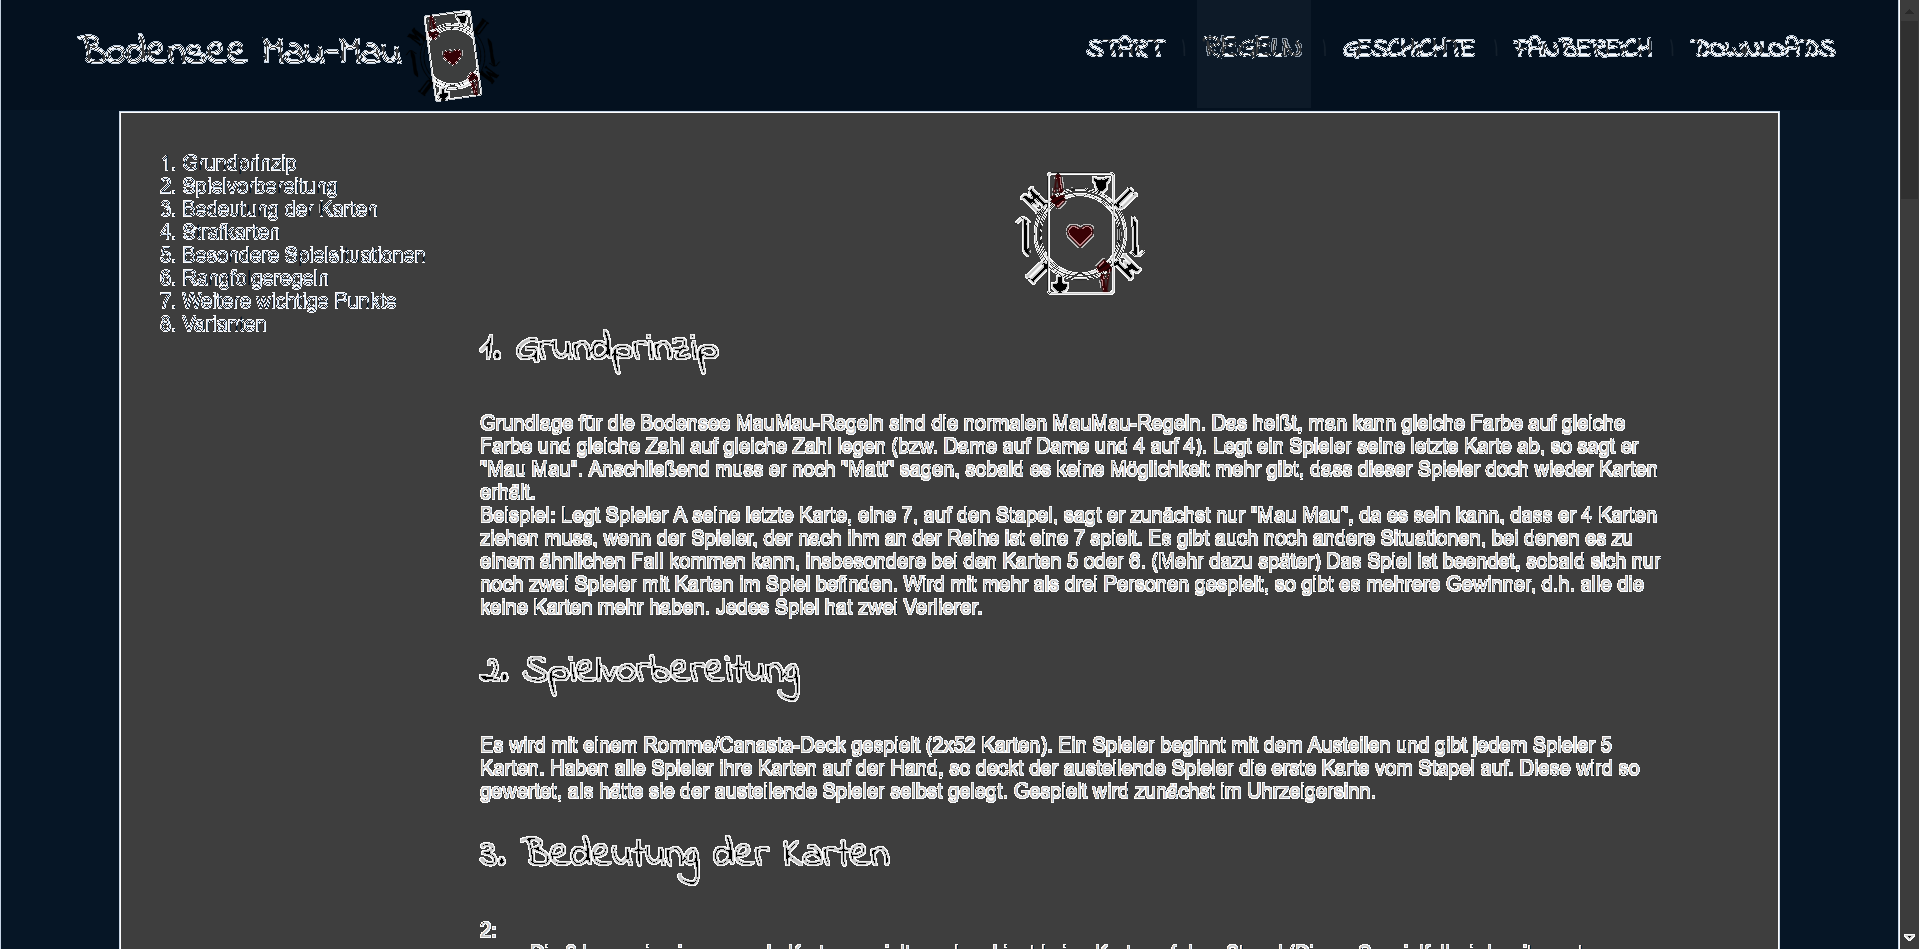
\includegraphics[width=300px, height=150px]{contrast.png}
\caption{Kontrastteset}
\end{figure}


Für Lesbarkeit und Orientierung ist der farblicher Kontrast ausreichend.



\section*{Aufgabe 9: Nutzertest}
Für den Nutzertest wurde \textbf{WebsiteV2} verwendet, bei der die Alternativtexte der Bilder auf der Seite \textit{Regeln} geändert wurden, so dass sie jetzt Sinn ergeben.

\begin{enumerate}
\item Wir haben uns die Fragestellung \textbf{"Wie kommen Erstnutzer mit der Seite zurecht?"} überlegt und wollten dabei testen, ob Szenario 2 (die Suche einer speziellen Regel) und Szenario 3 (aktuellste News abrufen) bewältigt werden können.
\item Wir haben ein Skript vorbereitet, das wir nach einem Pilottest leicht angepasst haben (nach Task 6 dürfen die Probanden noch die Webseite frei durchschauen). In \textbf{Abbildung 1} sieht man den Testraum.
\begin{description}
\item[Raum vorbereiten:]
Maus bereitstellen, Website öffnen, Aufnahmemodus (Win+G), restlichen Programme schließen
\item[Nutzer einweisen:]
Begrüßung und allgemeine Einweisung:
\begin{itemize}
\item Es geht um Website für ein Kartenspiel, mehr erfährst du während des Tests, bei dem ich dir Fragen/Aufgaben stellen werde, die du ausführen sollst und du sollst dabei alles laut aussprechen, was du denkst (Thinking Aloud)
\item Es geht darum die Website auf Probleme/Optimierungsmöglichkeiten zu prüfen und nicht darum den Tester zu prüfen, deswegen alles ohne Rücksicht sagen
\item Wir nehmen deinen Bildschirm auf (also die Mausbewegungen) und unser Gespräch (Audio), ist das okay?
\item Du darfst während des Tests Fragen stellen, aber es kann sein, dass ich sie nicht beantworten werde
\item Jetzt hast du nochmal die Möglichkeit Fragen zu stellen, bevor der Test beginnt
\end{itemize}
\textbf{Aufnahme starten}
  
\item[Aufgaben/Fragen stellen:]\ 
\begin{description}
\item[Task 1] Verschaff dir einen Überblick auf der Startseite, wenn du fertig bist, fangen wir an.
\item[Task 2] Finde die Regel zu der Spielkarte "Dame".
\item[Task 3] Lade einen Flyer herunter.
\item[Task 4] Was wurde als neustes auf der Website hinzugefügt?
\item[Task 5] Schreibe uns eine E-Mail.
\item[Task 6] Wie heißen die Gründer des Spiels?
\end{description}
Der Test ist zu Ende, jetzt darfst du selbständig schauen, ob du noch was findest.
\item[Ende:] Für die Teilnahme bedanken, Aufnahme beenden.
\end{description} 
\begin{figure}[H]
 \centering
   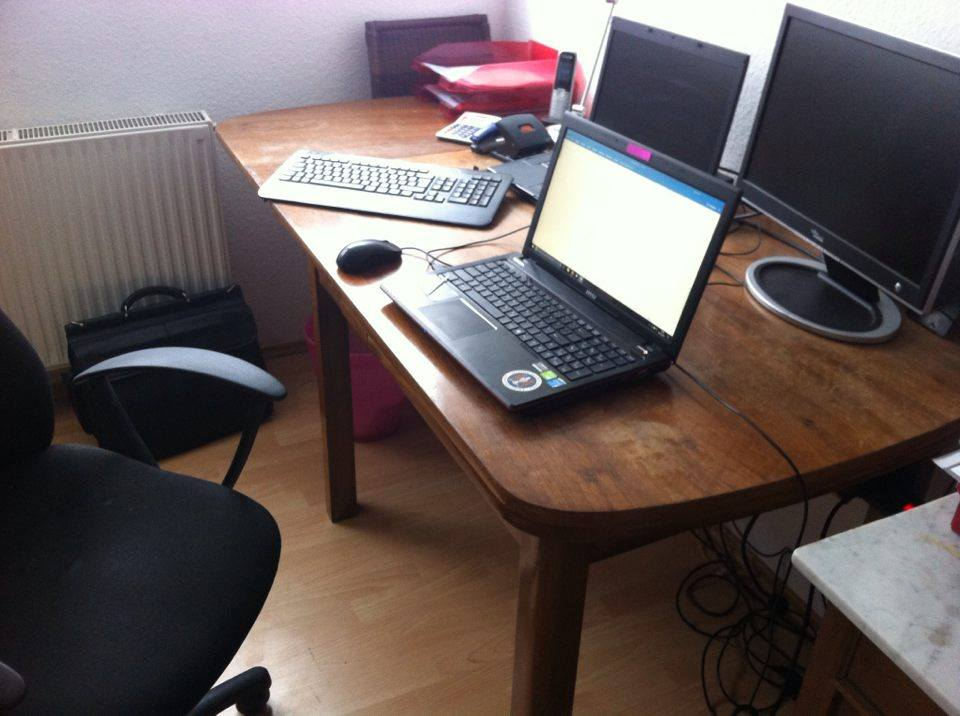
\includegraphics[width=0.7\textwidth]{nutzertest.jpg}
\caption{Raumvorbereitung für den Nutzertest}
\end{figure}
\item Wir haben 6 Probanden gefunden, inklusive Pilottest. Wir haben eigentlich keinen Protokollanten benötigt, da wir den Bildschirm und das Gespräch aufgenommen haben. Nur nachdem wir alle Tasks durchgeführt hatten, haben wir die vorgeschlagenen Verbesserungen der Probanden aufgeschrieben (als Anhang in \textbf{Protokoll.pdf}).
\item Für die Auswertung haben wir die Screenvideos nacheinander evaluiert und dabei die benötigte Bearbeitungszeit notiert, sowie alle Verbesserungsmöglichkeiten, die uns dabei aufgefallen sind.
\begin{description}
\item[Task 1] \textbf{Verschaff dir einen Überblick auf der Startseite. }\\
Das war keine wirkliche Aufgabe, wir wollten nur sicherstellen, dass die Probanden sich selbst einen Überblick nur mit der Startseite verschaffen, wie ein Erstnutzer es auch machen würde.
\item[Task 2] \textbf{Finde die Regel zu der Spielkarte Dame. }\\
Für diese Aufgabe kamen teilweise die längste Bearbeitungszeiten heraus (siehe Boxplot). Diese Aufgabe testet das Szenario 2.
\item[Task 3] \textbf{Lade einen Flyer herunter.} \\
Hier kamen kaum Anmerkungen zustande und es ging bei allen schnell und intuitiv.
\item[Task 4] \textbf{Was wurde als neustes auf der Website hinzugefügt?}\\ Das ging bei fast allen sehr schnell. Diese Aufgabe testet das Szenario 3.
\item[Task 5] \textbf{Schreibe uns eine E-Mail.}\\
Hier haben wir jede gefundene E-Mail-Adresse gelten lassen. Es wurden 3 verschiedene gefunden.
\item[Task 6] \textbf{Wie heißen die Gründer des Spiels?}\\
Das ging auch sehr schnell, manche haben diese Aufgabe über die Startseite und manche über die \textit{Geschichte}-Seite gelöst.
\end{description}

\subsection*{Themenblöcke:}
Prioritätenskala: 1 - 7 \\
sehr hohe Priorität = 1 und keine Priorität = 7
\begin{description}
\item[1. Eindeutigkeit] \
\begin{enumerate} 
\item Kontakt in Impressum zu finden nicht offensichtlich [6]
\item im Impressum sind zwei verschiedene E-Mail-Adressen und in Fanbereich eine dritte [2]
\item "Bedeutung der Karten"\ in "Kartenregeln"\ umbennen [3]
\end{enumerate}
\item[2. Entspricht nicht der Logik des Probanden] \
\begin{enumerate} 
\item das Wort Impressum war einem Probanden nicht bekannt [7]
\item Pfeil auf \textit{Geschichte}-Seite falschrum in der Logik eines Probanden [7]
\end{enumerate}
\item[3. Usability-Verbesserungsmöglichkeiten] \
\begin{enumerate}
\item Suchfeld in der linken Navigation auf der \textit{Regeln}-Seite [3]
\item Schlagwörter in den Regeln (manche Wörter hervorheben, um es übersichtlicher zumachen) [2]
\item Schrift leicht zu dünn in der Navigation [5]
\item Regeln haben viel Text [6]
\item Startseite, der Infotext ist nicht aussagekräftig genug [2]
\item Direkt Drucken - Button bei \textit{Downloads} [7]
\end{enumerate}
\item[4. Ausblick (große Verbesserungsmöglichkeiten)] \
\begin{enumerate}
\item Navigation mit 3 Strichen (mobile Version) [7]
\item Kartenbeispiele auf der \textit{Regeln}-Seite visuell darstellen [7]
\item Online spielen (gegen z. B. Computer, aber auch gegen andere Spieler) [7]
\end{enumerate}
\end{description}
\subsection*{Lösungen}
\begin{description}
\item[1b)] Alle E-Mail-Adressen wurden zu einer E-Mail-Adresse geändert und es gibt nur noch einen Kontakt-Bereich im Impressum.
\item[1c)] Der Titel "Bedeutung der Karten" wurde in "Kartenregeln" geändert.
\item[3a)] Ein Suchfeld kann noch in die linke Navigation auf der \textit{Regeln}-Seite hinzugefügt werden, doch leider erst mit JavaScript, was wir nicht verwenden dürfen, von daher lassen wir es lieber komplett draußen, damit wir nicht ein nicht-funktionierendes Suchfeld implementieren.
\item[3b)] Es wurde versucht den Regeln-Text durch kürzen und durch Hervorhebungen zu verbessern.
\item[3e)] Der Infotext auf der Startseite wurde auch angepasst.
\end{description}
\end{enumerate}
\subsection*{Bewertungsbericht}
Der Nutzertest lief im allgemeinen gut. Die Bearbeitungszeiten sind recht kurz gewesen, wie in den Boxplots erkennbar: \\ \\
\begin{tikzpicture}
  \begin{axis}
    [
    xlabel={Bearbeitungsdauer [in s]},
    ytick={1,2,3,4,5,6},
    yticklabels={Task 1, Task 2, Task 3, Task 4, Task 5, Task 6},
    ]
    \addplot+[
    boxplot prepared={
      median=57,
      upper quartile=45.5,
      lower quartile=64.75,
      upper whisker=70,
      lower whisker=23
    },
    ] coordinates {};
    \addplot+[
    boxplot prepared={
      median=35.5,
      upper quartile=66.25,
      lower quartile=14,
      upper whisker=67,
      lower whisker=14
    },
    ] coordinates {};
    \addplot+[
    boxplot prepared={
      median=9.5,
      upper quartile=11,
      lower quartile=7.5,
      upper whisker=14,
      lower whisker=6
    },
    ] coordinates {};
    \addplot+[
    boxplot prepared={
      median=14.5,
      upper quartile=23.75,
      lower quartile=9.5,
      upper whisker=29,
      lower whisker=5
    },
    ] coordinates {};
    \addplot+[
    boxplot prepared={
      median=15.5,
      upper quartile=22.25,
      lower quartile=9.5,
      upper whisker=23,
      lower whisker=2
    },
    ] coordinates {};
    \addplot+[
    boxplot prepared={
      median=10,
      upper quartile=3.75,
      lower quartile=13.5,
      upper whisker=18,
      lower whisker=3
    },
    ] coordinates {};
  \end{axis}
\end{tikzpicture}
\\
Da der erste Task keine richtige Aufgabe war, fällt eigentlich nur Task 2 aus dem Rahmen, vorallem auch aus der erwareteten Bearbeitungszeit. Die einfache Aufgabe, die Regel zur Spielkarte "Dame"\ zu finden, wurde für manche schwerer als erwartet, bzw. hat länger gedauert als erwartet. Dies soll durch die Lösungen zu den Problemen \textbf{1a)}, \textbf{3a)} und \textbf{3b)} behoben werden. \\
Gravierende Probleme wurden nicht gefunden, nur Optimierungsmöglichkeiten und kleine Uneindeutigkeiten. Alles in allem sind wir zufrieden, wie die Probanden sich auf der Webseite zurecht gefunden haben. Gelobt wurde, dass alles Wichtige da sei, das Logo kreativ sei und auch die \textit{Geschichte}-Seite schön sei, sowie der \textit{Über uns} - Bereich, der die Seite "weniger anonym, dafür persönlicher"\ machen würde.
\section*{Aufgabe 10: Projektabschluss}
 Halten Sie alles, was Sie darüber hinaus noch ändern im Abschlusskommentar fest. Geben Sie
an dieser Stelle einen kurzen Ausblick, welche Erweiterungsmöglichkeiten / Verbesserungen in
der Zukunft noch umgesetzt werden könnten. Begründen Sie, warum Ihre Webseite eine gute
Implementation Ihrer Projektidee ist.
 \subsection*{Ausblick} 
 Mobilversion, Design nochmal ordentlich überarbeiten?, Texte aktualisieren, Genderneutral umschreiben, Fremdsprachen hinzufügen,
 Fanstore, Onlineversion gegen PC und echte Spieler, Suchfeld in Regeln, mehr Icons für die Regeln, Bilder die Spiel erklären, Videos die Spiel erklären
 \subsection*{Fehlende Umsetzung}


\end{document}